%%%%%%%%%%%%%%%%%%%%%
%   AMS packages    %
%%%%%%%%%%%%%%%%%%%%%
\documentclass{amsart}

\usepackage{amsmath}
\usepackage{amsxtra}
\usepackage{amscd}
\usepackage{amsthm}
\usepackage{amsfonts}
\usepackage{amssymb}
\usepackage{eucal}
\usepackage[all]{xy}
\usepackage{graphicx}
\usepackage{tikz-cd}
\usepackage{mathrsfs}
\usepackage{subfiles}
%\usepackage{mathpazo} not a huge fan
\usepackage{euler}
\usepackage{hyperref}
\usepackage{color}
\usepackage{longtable}
\usepackage{float}

\usepackage[colorinlistoftodos, textsize=tiny]{todonotes}
\def\listtodoname{List of Todos}
\def\listoftodos{\@starttoc{tdo}\listtodoname}

%\addtolength{\oddsidemargin}{-.5 in}
	%\addtolength{\evensidemargin}{-.4 in}
	%\addtolength{\textwidth}{1 in}
%
	%\addtolength{\topmargin}{0 in}
	%\addtolength{\textheight}{0 in}

\RequirePackage{color}
\definecolor{myred}{rgb}{0.75,0,0}
\definecolor{mygreen}{rgb}{0,0.5,0}
\definecolor{myblue}{rgb}{0,0,0.65}

%\usepackage{hyperref}
  %\hypersetup{colorlinks=true,citecolor=blue}

\usepackage{tikz}
\usepackage{tikz-cd}
\usetikzlibrary{matrix,arrows,decorations.pathmorphing}

%%%%%%%%%%%%%%%%%%%%%%% amsthm theorem styles %%%%%%%%
%%%%%%%%%%%%%%%

\theoremstyle{plain}
  \newtheorem{thm}{Theorem}[section]
  \newtheorem{prop}[thm]{Proposition}
  \newtheorem{lem}[thm]{Lemma}
  \newtheorem{cor}[thm]{Corollary}
	\newtheorem{claim}[thm]{Claim}
	\newtheorem{question}[thm]{Question}
	
\theoremstyle{definition}
  \newtheorem{defn}[thm]{Definition}
  \newtheorem{example}[thm]{Example}
  \newtheorem{exer}[thm]{Exercise}
  \newtheorem{ctexample}[thm]{Counterexample}
  \newtheorem{convention}[thm]{Convention}
	\newtheorem{conjecture}[thm]{Conjecture}
	
\theoremstyle{remark}
	\newtheorem{rem}[thm]{Remark}
  \newtheorem{note}[thm]{Notation}
  \newtheorem*{note*}{Notation}
  \newtheorem{case}{Case}
	
\numberwithin{equation}{section}

%%%%%%%%%%%%%%%%%%%%%%%%% custom commands %%%%%%%%%%%%%%%%%%%%%%%%%%%

\newcommand\nc{\newcommand}
\nc\on{\operatorname}
\nc\renc{\renewcommand}
\newcommand\ssec{\subsection}
\newcommand\sssec{\subsubsection}
\newcommand\BH{{\mathbb H}}
\newcommand\bO{{\mathbf O}}
\newcommand\CC{{\mathcal C}}
\newcommand\BN{{\mathbb N}}
\newcommand\BC{{\mathbb C}}
\newcommand\BF{{\mathbb F}}
\newcommand\BR{{\mathbb R}}
\newcommand\BQ{{\mathbb Q}}
\newcommand\BP{{\mathbb P}}
\newcommand\BBZ{{\mathbb Z}}
\newcommand\uR{\underline{R}}
\newcommand\uZ{\underline{\BBZ}}
\newcommand\CF{{\mathcal F}}
\newcommand\uCF{\underline{{\mathcal F}}}
\newcommand\BZ{{\mathbb Z}}
\newcommand\BA{{\mathbb A}}
\newcommand\fa{{\mathfrak a}}
\newcommand\fp{{\mathfrak p}}
\newcommand\fq{{\mathfrak q}}
\newcommand\fm{{\mathfrak m}}
\newcommand\so{{\mathscr O}}
\newcommand\sg{{\mathscr G}}
\newcommand \sx{\mathscr X}

\newcommand\scm{{\mathscr M}}
\newcommand\scn{{\mathscr N}}
\newcommand\scf{{\mathscr F}}
\newcommand\scg{{\mathscr G}}
\newcommand\sco{{\mathscr O}}
\newcommand\sch{{\mathscr H}}
\newcommand\scl{{\mathscr L}}
\newcommand\sci{{\mathscr I}}

\newcommand{\id}{\mathrm{id}}
\newcommand\im{\text{im }}
\newcommand\coker{\text{coker}}
\newcommand \spec{\text{Spec }}
\newcommand \proj{\text{Proj }}
\newcommand \rspec{\textit{Spec }}
\newcommand \rproj{\textit{Proj }}
\newcommand{\gal}{\mathrm{Gal}}

\newcommand \trdeg{\text{tr. deg }}
\newcommand \codim{\text{codim}}
\newcommand \rk{\text{rk }}
\newcommand \di{\text{Div }}
\newcommand \depth{\text{depth }}
\DeclareMathOperator{\ord}{ord}
\DeclareMathOperator{\sym}{Sym}

%%%%%%%%%%%%%%%%%%%%% cring custom commands %%%%%%%%%%%%%%%%%%%%%%%%%

\newcommand \subhalf[1]{\frac{{#1} - 1}{2{#1}}}
\newcommand{\se}[1]{\section*{Problem #1}}
\newcommand \halfcan{L}
\newcommand \Supp{\text{Supp}}
\newcommand \initial{\text{in}}
\newcommand \gin{\text{gin}}
\newcommand \Eff{\text{Eff}}
\newcommand \sat{\text{sat}}

%%%%%%%%%%%%%%%%%%%%%%%%%%%%%% title %%%%%%%%%%%%%%%%%%%%%%%%%%%%%%%%

\title{Spin canonical divisors of log stacky curves}

\author{Aaron Landesman}
\address[Aaron Landesman]{Department of Mathematics, Harvard University}
\email{aaronlandesman@college.harvard.edu}

\author{Peter Ruhm}
\address[Peter Ruhm]{Department of Mathematics, Stanford University}
\email{pruhm@stanford.edu}

\author{Robin Zhang}
\address[Robin Zhang]{Department of Mathematics, Stanford University}
\email{robinz16@stanford.edu}

\date{\today}

%%%%%%%%%%%%%%%%%%%%%%%%%%%%% document %%%%%%%%%%%%%%%%%%%%%%%%%%%%%%

\begin{document}


\maketitle

\begin{abstract}
  Generalizing the classical theorems of Max Noether and Karl 
	Petri, we describe generators and relations for the spin canonical
	ring of a stacky curve equipped with an arbitrary log divisor. As
	an application, we bound the generation degrees and relation
	degrees for graded rings of modular forms of arbitrary integral
	weight arising from finite-area quotients of the upper half-
	plane by Fuchsian groups.
\end{abstract}

\todo{Peter: I don't like the first thing our reader will read to be a dependent clause}

%%%%%%%%%%%%%%%%%%%%%%%%%%%% Introduction %%%%%%%%%%%%%%%%%%%%%%%%%%%%%%%

\section{Introduction}
Let $\Gamma$ be a {\bf Fuchsian} group, i.e. a discrete subgroup
of $PSL_2(\BR)$ acting on the upper half plane $\BH$ by fractional
linear transformations. We consider the {\bf ring of modular forms}
$M(\Gamma) = \bigoplus_k M_k(\Gamma)$. In this paper, we sharply bound the degree of the generators and
relations for $M(\Gamma)$, for general $\Gamma$ \todo{Peter: Why do you say general gamma?  I think you should either add "general fuchsian groups gamma" or just take out that clause, since you just defined what gamma is.}  \todo{Peter: also, its not clear to me that this should be said right here.  I think we may want to say a bit more about what's already known instead of going directly to what we have done}.  In the special that $\Gamma$ has no odd weight modular forms, Voight and Zureick-Brown
\cite[Chapters 7-9]{vzb:stacky} give similar bounds, and we extend their work to all Fuchsian groups $\Gamma$. In order to find generators and relations for $M(\Gamma)$, we translate the seemingly analytic question of understanding the ring of modular forms into the algebraic
category, using a generalization of the GAGA principle. By
\cite[Proposition 6.1.5]{vzb:stacky}, there is an equivalence of
categories between orbifold curves and log stacky curves over $\BC$
. Hence, for the remainder of the paper, we will work in the
algebraic category.

Let $X$ be a smooth algebraic curve over $k$ of genus $g$. It is
well known that the canonical sheaf $\Omega _X,$ with associated canonical divisor $K_X$
 determines the {\bf canonical map } $\pi:X \rightarrow \BP_k^{g - 1}$.
Then, the {\bf canonical ring} is defined to be
\begin{align*}
	R(X,K_X) = \bigoplus_{d \geq 0} H^0(X, dK_X),
\end{align*}

\noindent
with multiplication structure corresponding to tensor product of
sections. In the case that $g \geq 2$, $\Omega_X$ is ample, so $X \cong \proj R$. When $g \geq 2$, Petri's
theorem gives generators and relations for $R(X, K_X)$ showing that
in most cases $R(X, K_X)$ is generated in degree 1 with relations
in degree 2 (one demonstration is given by Saint-Donat\cite[p. 157]{saint-donat:proj}). This has the
pleasant geometric consequence that all such canonically embedded
curves are scheme theoretically cut out by quadratic equations.

\todo{Peter: I think we need something about odd weight modular forms before going right into stacks.}  
Following Voight and Zureick-Brown \cite{vzb:stacky}, we generalize Petri's theorem in many \todo{Peter: not clear to me that ``many'' is a good word to use here.  We mostly generalize in one direction}
directions. 
If $X$ is a curve, \todo{why do you start with a curve and then move to a stacky curve? shouldn't it be the opposite order?} then we say $\sx$ is a {\bf stacky curve} with {\bf coarse space} $X$ and {\bf stacky points} $P_1,\ldots, P_r$ with {\bf stabilizer orders} $e_1,\ldots, e_r \in \BZ_{\geq 2}$ if 
$$\di \sx = \di X \oplus \left(\bigoplus_{i
= 1}^r \left\langle \frac{1}{e_i}P_i \right\rangle \right) \subset \BQ \otimes \di X.$$
As is done in Voight and Zureick-Brown \cite{vzb:stacky} one may view a stacky curve as a stack, but for the purposes of this paper, it suffices to view $\sx$ as a scheme whose associated divisor group allows a finite number of ``fractional points,'' i.e., stacky points. A {\bf log spin curve} is a triple $(\sx, \Delta, \halfcan)$ where $\Delta \in \di X$ is an effective divisor and $2\halfcan = K_X + \Delta + \sum_{i=1}^{r}\subhalf{e_i}P_i.$
The central object of study in this paper is the {\bf log spin
canonical ring} of $(\sx, \Delta, \halfcan)$ is
\begin{align*}
	R(\sx, \Delta, \halfcan) = \bigoplus_{d \geq 0} H^0(\sx,\lfloor d \halfcan \rfloor)
\end{align*}

In particular, we would like to bound the degrees in which the
graded ring and its relations are generated. The work by O'Dorney
shows that the canonical ring of any $\BQ$-divisor $D =
\frac{\alpha_1}{\beta_1}P_1 + \frac{\alpha_2}{\beta_2}P_2$ of
$\BP_k^1$ with $\# \Supp(D) \leq 2$ is generated in degrees up
to $e := \max(\beta_1, \beta_2)$ with relations generated in
degrees up to $2e$ \cite[Section 4]{dorney:canonical}. Furthermore,
O'Dorney gives a larger bound when the support of $D$ is allowed to
have arbitrarily many points in terms of least-common-multiples.
Voight and Zureick-Brown also bounded the generator and relation
degrees of log spin canonical rings of $(\sx, \Delta, \halfcan)$,
in the case that genus is positive and $\halfcan$ is effective,
by $3e$ and $6e$ for $e := \max(e_1, \ldots, e_r)$.

The goal of this paper is to provide a stricter bound on the
generator and relation degrees of log spin canonical rings
for all genera. Note that O'Dorney's bounds are asymptotically
strict for arbitrary $\BQ$-divisors on $\BP^1$, but restricting
to the log spin curve case allows for lower bounds.
The main theorem of this paper is the following improved bound on
the degree of generators and relations of log spin canonical rings:

\todo{State for even weight modular forms attributed to VZB.}
\begin{thm}
\label{thm:main}
Let $(\sx, \Delta, \halfcan)$ be a log spin curve over a perfect field $k$, \todo{Ask David: do we need this perfectness assumption everywhere?} so
that $\sx$ has signature $\sigma = (0; e_1, \ldots, e_r; \delta)$. Then the
canonical ring

\begin{align*}
	R(\sx, \Delta, \halfcan) = \bigoplus_{d \geq 0} H^0(\sx, \lfloor d \halfcan \rfloor)
\end{align*}

\noindent
is generated as a $k$-algebra by elements of degree at most $e =
\max(5, e_1, \ldots, e_r).$ If the genus $g \geq 2,$ and $\Delta = 0
$ then $R(\sx,\Delta, \halfcan)$ has relations generated in degrees
up to $\max(11, 2e_1, \ldots, 2e_r)$. Otherwise, $R(\sx, \Delta,
\halfcan)$ has relations generated in degrees up to $\max(10, 2e_1,
\ldots, 2e_r),$ so long as $\sigma$ does not lie in a finite list
of exceptional cases, as listed in Table ~\ref{table:g-1-exceptional}
for signatures with $g = 1$ and Table ~\ref{table:g-0-exceptional}
for signatures with $g = 0$.
\end{thm}

This theorem is proven in three different genus cases, each of
which use similar inductive processes. The genus $g \geq 2$ case is
proven in Theorem ~\ref{thm:g-high-main}. In Theorem
~\ref{thm:g-1-main} and Theorem
~\ref{thm:g-0-main}, we also give the respective
genus one and genus zero results after using a similar induction
process while dealing with more complicated base cases and
exceptional cases.

\begin{rem}
\label{rem:explicit-generators}
The proofs of the main theorems in the low genus cases not only
obtain bounds on the degrees of the generators and relations, but
also yield explicit systems of generators and the initial ideal of
relations. Furthermore, our proof of the high genus case also
provides an inductive procedure for determining the generators and
initial ideal of relations for the half-canonical divisor $\halfcan$
 can be written as $\halfcan = \halfcan' + \Lambda$ with $(\halfcan
', \Delta, \sx)$ when $\Lambda \in \di \sx$ effective. In fact,
such a system of generators and relations are known for $\halfcan'$
in many interesting low genus cases, as detailed in Neves
~\cite[Section III.4]{neves:halfcan}.
\end{rem}

The main theorem of this paper provides the following application
to modular forms when combined with a result from Voight and
Zureick-Brown ~\cite[Lemma 10.2.1]{vzb:stacky}.

\begin{cor}
\label{cor:main-mod-forms}
Let $\Gamma$ be a Fuchsian group and $\sx$ the stacky curve
associated to $\Gamma \backslash \BH$ with signature $(g; e_1,
\ldots, e_r; \delta)$. Then the ring of modular forms
$M(\Gamma) := \bigoplus_{k = 0}^{\infty} M_k(\Gamma)$ is
generated as a $\BC$-algebra by elements of degree at most $e = \max
 (5$, $e_1$, $\ldots$, $e_r).$ If the genus $g \geq 2,$ and $\Delta = 0$
then $M(\Gamma)$ has relations generated in degrees up to $\max(11,
2e_1, \ldots, 2e_r)$. Otherwise, $M(\Gamma)$ has relations
generated in degrees up to $\max(10, 2e_1, \ldots, 2e_r)$, so long
as $\sigma$ does not lie in a finite list of exceptional cases, as
listed in Table ~\ref{table:g-1-exceptional} for signatures with $g
= 1$ and Table ~\ref{table:g-0-exceptional} for signatures with $g =
0$.
\end{cor}

The remainder of the paper will be primarily devoted to proving
Theorem ~\ref{thm:main}. The idea of the
proof will be to induct on the stabilizer order of and number of stacky points. To this end, we first review important background in
Section ~\ref{sec:background}. Then, we develop various inductive
tools in Section ~\ref{sec:induction}. In Sections ~\ref{sec:g_high},
~\ref{sec:g_1}, and ~\ref{sec:g_0}, we prove Theorem
~\ref{thm:main} in the high genus, genus
one, and genus zero cases respectively. Finally, in Section
~\ref{sec:further-questions}, we pose several questions for future
research.

%%%%%%%%%%%%%%%%%%%%%%%%%%%% Background %%%%%%%%%%%%%%%%%%%%%%%%%%%%%%%

\todo{Somewhere in the paper, we should probably give an example showing the generators and relations are sharply bounded at degree e, 2e. Robin: Aren't the base cases suitable examples? Aaron: Those don't show it for general e, do they? I don't think we really need an example, just a remark somewhere that one cannot really hope to do better than e, 2e somewhere.}

\section{Background}
\label{sec:background}
Here we denote various definitions and useful notation that will be
used throughout the paper. Many of the conventions come from existing
literature. For basic references on the statements and definitions
used below, see Hartshorne \cite[Chapter IV]{hartshorne:ag},
Saint-Donat \cite{saint-donat:proj}, the book of Arbarello--
Cornalba--Griffiths--Harris \cite[Section III.2]
{acgh:algebraic-curves}, and Voight--Zureick-Brown \cite[Chapter 2,
Chapter 5]{vzb:stacky}.

\ssec{Stacky Curves and Log Spin Canonical Rings}
\label{ssec:stacky-background}
A \textbf{stacky curve} $\sx$ over a field $k$ is a smooth proper
geometrically-connected Deligne-Mumford stack of dimension $1$ over
$k$ with a dense open subscheme. A stacky curve is \textbf{tame} if
its stabilizers are coprime to char $k$. Throughout this paper,
stacky curves will be assumed to be tame and $k$ will always be
algebraically closed. The language of stacks will be omitted in
this paper, as it is sufficient to view stacky curves and related
objects $\sx$ as a scheme whose associated divisor group allows for
a finite number of \textbf{stacky points} which may be viewed
heuristically as ``fractional points''. See Voight and
Zureick-Brown for more thorough treatment of these definitions
\cite[Chapter 5]{vzb:stacky}.

If $P_1, \ldots, P_r$ are the stacky points of a stacky curve $\sx$,
then we use $e_1,\ldots, e_r \in \BZ_{\geq 2}$ to denote the orders
of the stabilizer groups of the points with non-trivial
stabilizers. We call $e_i$ the \textbf{stabilizer order} of $P_i$.
In order to study objects associated with stacky curves, it is often
useful to consider them in the context of ordinary schemes. 

\begin{defn}
Let $\sx$ be a stacky curve over $k$ with stacky points $P_1, \ldots,
P_r$ with stabilizer orders $e_1,\ldots, e_r \in \BZ_{\geq 2}$.
Let $X$ be a nonsingular projective (algebraic) curve over $k$ of
genus $g$. Then $X$ is the \textbf{coarse space} associated to $\sx$
if

\[
	\di \sx = \di X \oplus \left(\bigoplus_{i
	= 1}^r \left\langle \frac{1}{e_i}P_i \right\rangle \right) \subset \BQ \otimes \di X
\]
\end{defn}

We can equip stacky curves with a divisor $\Delta$ that is a 
sum of distinct points each with trivial stabilizer. A divisor
$\Delta$ of this form is called a \textbf{log divisor}. We use
$\delta := \deg \Delta$ to refer to the degree of the log divisor.
If $\sx$ has coarse space $X$ of genus $g$, then we say $\sx$ has
\textbf{signature} $\sigma = (g; e_1, \ldots, e_r; \delta)$.

The pairs $(\sx, \Delta)$ are called \textbf{log stacky curves}
and the study of their canonical rings is the main focus of
the work by Voight and Zureick-Brown \cite{vzb:stacky}.
For this paper, we consider \textbf{log spin curves} which are
triples $(\sx, \Delta, \halfcan)$ where $\Delta$ is a log divisor
and a divisor $\halfcan$ which satisfies the property that
$2\halfcan \sim K_\sx + \Delta$. Such a divisor $\halfcan$
is called a \textbf{half-canonical divisor} on $(\sx, \Delta)$
and are sometimes referred to as theta-characteristics in other
literature. We also use $\halfcan_X$ to refer to the half-canonical
divisor associated with the coarse space $X$ of $\sx$, i.e.
$\halfcan_X$ is a divisor such that $2\halfcan \sim K_X$.
Now we can define the analogy to canonical rings for
log spin curves.

\begin{defn}
If divisor $D \in \di \sx$ and $D = \sum_{i = 1}^{n} \alpha_i P_i$
with $\alpha_i \in \BQ$, the floor of a divisor $\lfloor D
\rfloor$ is defined to be $\lfloor D \rfloor := \sum_{i = 1}^{n}
\lfloor \alpha_i \rfloor P_i$.

The {\bf log spin canonical ring} of $(\sx, \Delta, \halfcan)$ is
\[
	R(\sx, \Delta, \halfcan) = \bigoplus_{d \geq 0} H^0(\sx, \lfloor d \halfcan \rfloor)
\]
\end{defn}

\noindent
When the log spin curve is fixed, we usually use $R$ or $R_L$ to
represent $R(\sx, \Delta, \halfcan)$. We also often use $H^0(\sx, D)
:= H^0(\sx, \sco(D))$ and $h^0(\sx, \sco(D)) := \dim H^0(\sx, \sco(D))$.

\todo{do this part}
Part on Kodaira--Spencer \cite{kodaira:complex-manifolds}.


\todo{Note that this result is independence of base field}

If $R$ is a graded ring, then $(R)_d$ refers to the $d^{th}$ degree
component of $R$.

\begin{defn}
\label{def:order-sup}
If $z$ is a rational section of $\sco(D)$ denote the order of
zero of $z$ at $P$ by $\ord_P^D(z)$.
\end{defn}


\begin{rem}
\label{rem:odd-denom}
Suppose $(\sx, \Delta, L)$ is a log spin curve. Note that
\[
	L = \sum_{i = 1}^{r} \frac{e_i - 1}{2e_i} P_i + \sum_{i = 1}^{s} a_i P_i
\]

\noindent
where $a_i \in \BZ$ and $e_i$ are odd.
\todo{give reason}
\end{rem}
	
\begin{rem}
\label{rem:delta-not-1}
Suppose $(\sx,\Delta,L)$ is a log spin curve. Note that $\deg \Delta
$ is even. because $2 \cdot \deg L = \deg \Delta + \deg \lfloor K
\rfloor = \deg \Delta + 2(g-1).$ Therefore, $\deg \Delta$ is even.
In particular, we shall often use $\deg \Delta \neq 1$.
\end{rem}


We define the notion of the saturation of a divisor, taken from
Voight and Zureick-Brown ~\cite[Section 7.2]{vzb:stacky}.

\begin{defn}
Let $D$ be a divisor on $\sx$. The \textbf{effective monoid} of $D$
is the monoid
\[
	\Eff(D) = \{d \in \BZ_{\geq 0} : \deg \lfloor dD \rfloor \geq 0 \}
\]
\end{defn}

\begin{defn}
\label{defn:sat}
The \textbf{saturation} for a monoid $M \subseteq \BZ_{\geq 0}$,
denoted $\sat(M)$, is the smallest integer $s$ such that $M
\supseteq \BZ_{\geq s}$, if such an integer exists.
\end{defn}

\begin{rem}
For our purposes, it is useful to call the saturation of the
effective monoid of a divisor $D$ as the saturation $s$ of the
divisor $D$ on $\sx$. In this case, the saturation $s :=
\sat(\Eff(D))$ of a divisor $D$ on $\sx$ is the smallest positive
$s \in \BZ$ such that $\deg \lfloor dD \rfloor \geq 0$ for all $d
\geq s$.
\end{rem}

\ssec{Monomial Ordering}
\label{ssec:monomial-order}
Here we give a brief overview of the monomial orderings
that we use. For further reference on monomial orderings,
initial ideals, and Gr\"{o}bner bases, see Eisenbud
\cite[Section 15.9]{eisenbud:comm-alg} and Cox--Little--Shea
\cite[Chapter 2]{cls:ideals-varieties-algorithms}.

We equip the polynomial ring $k[x]_{\vec{a}}$ with the (weighted graded) reverse lexicographic order \defiindex{grevlex} $\prec$: if 
\[ x^{\vec{m}} = \prod_{d,i} x_{d,i}^{m_{d,i}} \]
and $x^{\vec{n}}$ are monomials in $k[x]_{\vec{a}}$, then $x^{\vec{m}} \succ x^{\vec{n}}$ if and only if either
\begin{equation}
\vec{a}\cdot\vec{m} = \sum_{d,i} dm_{d,i}  > \vec{a} \cdot \vec{n}
\end{equation}
or
\begin{equation} \label{eqn:grevlexdef}
\text{$\vec{a}\cdot\vec{m} = \vec{a} \cdot \vec{n}$ and the last (right-most) nonzero entry in $\vec{m}-\vec{n}$ is negative.}
\end{equation}
It is important to note that in \eqref{eqn:grevlexdef}, the ordering of the variables matters: it corresponds to a choice of writing the exponents of a monomial as a vector.  A common choice for us will be
\begin{equation} \label{eqn:xdOrder}
 x_{1,1}^{m_{1,1}} \cdots x_{D,a_D}^{m_{D,a_D}} \leftrightarrow (m_{D,1},\dots,m_{D,a_D},\ldots,m_{1,1},\dots,m_{1,a_1}) 
 \end{equation}
in which case we have $x_{2,1} \succ x_{1,2}^2$
and $x_{5,1} \succ x_{1,6}^2 x_{3,2}$, etc.
We indicate this ordering in the presentation of the ring, e.g.~for the above we would write
\[ k[x]_{\vec{a}}= k[x_{1,1},\dots,x_{1,a_1},\dots,x_{D,1},\dots,x_{D,a_D}]. \]
In this way, our relations write generators in larger degree in terms of those in smaller degree (``later generators in terms of earlier generators''), which gives the most natural-looking canonical rings to our eyes.

For a homogeneous polynomial $f \in k[x]_{\vec{a}}$, we define the \textbf{initial term} $\init_{\prec}(f)$ to be the monomial in the support of $f$ that is largest with respect to $\prec$, and we define $\init_{\prec}(0)=0$.  Let $I \subseteq k[x]_{\vec{a}}$ be a homogeneous ideal.  We define the \textbf{initial ideal} $\init_{\prec}(I)$ to be the ideal generated by $\{\init_{\prec}(f) : f \in I\}$.  A \textbf{Gr\"obner basis} (also called a \textbf{standard basis}) for $I$ is a set $\{f_1,\dots,f_n\} \subset I$ such that 
\[ \langle \init_{\prec}(f_1),\dots,\init_{\prec}(f_n) \rangle = \init_{\prec}(I). \]

A Gr\"obner basis for $I$ \emph{a priori} depends on a choice of basis for the ambient graded polynomial ring; we now see what happens for a general choice of basis.



background on Gr\"{o}bner bases
Notation for Gr\"{o}bner bases and orderings (include grlex, grevlex, and block order, as defined in \cite[Definition 8.1.1]{vzb:stacky})


\subsection{Junk}
This is stuff that has been moved out of the introduction to possibly
be retooled for this section.

We can then consider the
orbifold $\Gamma \backslash \BH$ over $\BC$. For example, in the
case $\Gamma$ acts freely on $\BH$, $\Gamma \backslash \BH$ is a
Riemann Surface over $\BC$. It may well be that $\Gamma \backslash
\BH$ is not compact. Defining $\Delta$ as the divisor of cusps
associated to $\Gamma$, we can form a space $\Gamma \backslash
\BH^*$ which is a compactification of $\Gamma \backslash \BH,$ with
associated {\bf divisor of cusps} $\Delta$.

%%%%%%%%%%%%%%%%%%%%%%%%%%% Inductive lemmas %%%%%%%%%%%%%%%%%%%%%%%%%%%%%%%


\section{Inductive Lemmas}
\label{sec:induction}
First we present several lemmas which provide the
inductive steps for the proof of the main theorem: Theorem
~\ref{thm:main}. In Subsection ~\ref{ssec:add-points} we prove three lemmas
%Lemma ~\ref {lem:sat-1}, ~\ref{lem:sat-2}, and ~\ref{lem:sat-3}
which determine the generators and relations of $R_\halfcan=R_{\halfcan' + \frac{\alpha
}{\beta}P}$ from those of $R_{\halfcan'}$, where
%where $X$ is a curve, \todo{Peter: I don't think we need to include this instantiation; $X$ always represents a curve throughout the paper, and we should say something to that effect in the background}
$\halfcan \in \di
X \otimes \BQ $ and  $\frac{\alpha}{\beta} \in \BQ$. 
In
Subsection ~\ref{ssec:raise-orders}, we prove a inductive lemma allowing us to transfer information about the log half canonical ring of a curve with signature $(g; e_1', 
\ldots, e_\tau'; 0)$ to that of a
curve with the same log divisor, the same stacky points, and some subset of the $e_ i'$ incremented by $2$. \todo{Peter: I tried to edit this, but I can't figure out how to make this sentence work well.  There are too many clauses...}
%While Lemma ~\ref{lem:sat-1} may be applied in a fairly general 
%context, Lemma ~\ref{lem:raise-stacky-order} is more specific to 
%half-canonical divisors.

%However, before we can answer these general lemmas, it is useful
%to prove a nice result about minimal generation of ideals of
%relations.
%
%\todo{Include one of the following, if the first one, include a 
%remark for quotient}

%\begin{lem}
%\label{lem:minimal_quadratic}
%Suppose $k[x_1, \ldots, x_n]$ is a graded ring, not necessarily
%generated in degree 1, is equipped with a monomial ordering $\prec$.
 %Let $\phi:k[x_1, \ldots, x_n] \rightarrow B'$ be a map of graded
%rings with kernel $I'$, such that $I'$ is generated by elements $f_1,
%\ldots, f_j$, where $in_\prec(f_i) = x_i x_j,$ and no term of $f_i$
%is of the form $x_k$. Then, the elements $f_i$ determine minimal
%generators for $I$.
%\end{lem}
%\begin{proof}
%Regrade the ring $k[x_1, \ldots, x_n]$ so that all $x_i$ lie in
%degree 1. Then,
%\[
	%\phi : k[x_1, \ldots, x_n] \rightarrow B
%\]
%\noindent
%determines a map of rings, no longer necessarily graded. Consider
%the grlex monomial ordering $\prec$ on $k[x_1, \ldots, x_n]$.
%\todo{This ordering isn't quite right. 
%We need to preserve the ordering on quadratic terms}
%By
%assumption, the kernel $I$ is generated by elements whose initial
%terms have degree 2 and are all distinct. Therefore, $\dim_k (k[x_1,
%\ldots, x_n])_2 = \binom{n}{2} - j.$ This implies any set of
%generators for $I$ must have at least $j$ elements. Since $f_1,
%\ldots, f_j$ is such a set, it is minimal.
%\end{proof}
%
%\begin{rem}
%In particular, in the case of
%\[
	%\begin{tikzcd}
		%I\ar[hookrightarrow]{r}\ar[hookrightarrow]{d} & k[x_1, \ldots, x_n]
		%\ar[twoheadrightarrow]{r} \ar[hookrightarrow]{d} & B \ar[hookrightarrow]{d} \\
		%I' \ar[hookrightarrow]{r} & k[x_1, \ldots, x_n, y_1, \ldots, y_m] \ar[twoheadrightarrow]{r}& B'
	%\end{tikzcd}
%\]
%inducing
%\[
	%I/I'\hookrightarrow k[y_1, \ldots, y_m]\twoheadrightarrow B'/B
%\]
%\todo{how do we make this proof?}
%\end{rem}
%\begin{lem}
%\label{lem:minimal_quadratic}
%Suppose $k[x_1, \ldots, x_n]\hookrightarrow k[x_1, \ldots, x_n, y_1, \ldots, y_m]$ be graded ring, not necessarily
%generated in degree 1 that are equipped with monomial ordering $\prec$.
%Let $\phi: k[x_1, \ldots, x_n] \twoheadrightarrow B, \phi':k[x_1, \ldots, x_n, y_1, \ldots, y_m]\twoheadrightarrow B'$ be maps of graded
%rings with kernels $I \hookrightarrow I'$ such that the following diagram commutes:
%\[
	%\begin{tikzcd}
	%I\ar[hookrightarrow]{r}\ar[hookrightarrow]{d} & k[x_1, \ldots, x_n]\ar[twoheadrightarrow]{r} \ar[hookrightarrow]{d} & B \ar[hookrightarrow]{d}\\
	%I' \ar[hookrightarrow]{r} & k[x_1, \ldots, x_n, y_1, \ldots, y_m] \ar[twoheadrightarrow]{r}& B'
	%\end{tikzcd}
%\]
%Further suppose that $I'$ is generated over $I$ by elements $f_1,
%\ldots, f_j$ as a $k$-vector space, where $in_\prec(f_i) \in \{y_i x_j, y_i y_j\}$ and no monomial of $f_i$
%is of the form $y_i$. Then, the elements $f_i$ determine minimal
%generators for $I'$ over $I$.
%\end{lem}
%
%\begin{proof}
%Regrade the rings $k[x_1, \ldots, x_n], k[x_1, \ldots, x_n, y_1, \ldots, y_m]$ so that all $x_i$ and $y_j$ lie in
%degree 1. Then,
%\[
	%\phi : k[x_1, \ldots, x_n] \twoheadrightarrow B 
%\]
%\[
	%\phi': k[x_1, \ldots, x_n, y_1, \ldots, y_m] \twoheadrightarrow B'
%\]
%
%
%\noindent
%determines map of rings, no longer necessarily graded. 
%By assumption, $I'$ is generated over $I$ as a $k$-vector space by elements $f_1, \ldots, f_n$ whose initial terms have degree 2 and are linearly independent. By the theory of Gr\"{o}bner basis,
%\[
	%\dim_k(B'/B)_2=\dim_k(k[x_1, \ldots, x_n, y_1, \ldots, y_m]/k[x_1, \ldots, x_n])_2 - j
%\]
%so
%\[
	%\dim_k (I'/I)_2=j.
%\]
%This implies any set of
%generators for $I$ must have at least $j$ elements. Since $f_1,
%\ldots, f_j$ is such a set, it is minimal.
%\end{proof}
%
%\begin{rem}
%\label{rem:minimal_quadratic_trivial_case}
%It will be useful to use Lemma ~\ref{lem:minimal_quadratic} in the
%case $m= 0$, in which case we find explicitly that $f_1, \ldots, f_r$
%are $k$-minimal generators for $I'$ (over the trivial base vector
%space). 
%\end{rem}
%With this result, we will be able to show that the sets of generators of the ideal of relations in many of the following inductive arguments are minimal.


\ssec{Adding Points}
\label{ssec:add-points}
%In this section, we prove various inductive statements under the following setup:
%Let $\halfcan' \in \di \BQ \otimes X$ be $\BQ$-divisor of $X$ (and often a log half-canonical divisor of some $\sx'$), satisfying certain conditions about $\deg(\lfloor d \halfcan'\rfloor)$ for various values of $d\in\mathbb{N}$ and certain saturation conditions. Let $\halfcan=\halfcan'+P$ for some $P$ possibly in the support of $\halfcan$.  Then we will explicitly describe elements that generate $R_\halfcan$ over $\halfcan$' and initial terms of relations that generate $\initial(I')$ over $\initial(I)$ (allowing the construction of a corresponding Gr\"{o}bner Basis). \todo{Aaron: What new ideas does this description add that wasn't already described in the previous paragraph? Also, in general it's a good idea to be specific about what the most important lemmas are in the section, although I also added this to the general description of section 3.}

Before proving three lemmas that allow us to inductively add points to the support of a divisor (i.e. $\halfcan\to \halfcan + \frac{\alpha}{\beta}P$), we give a criteria to determine if a set of monomials generates the initial ideal of relations of $k[x_1, \ldots, x_m]\to R_D$.  This will be used in three lemmas of this section to show, in each case, that a chosen homogeneous ideal is in fact the ideal of relations.\todo{Peter:This last sentence is a little redundant}


\begin{lem}\label{lem:relations_from_generators_induction} 
Suppose $\halfcan, \halfcan' \in \di X \otimes \BQ$ with $\halfcan=\halfcan'+\frac{\alpha}{\beta}P$, such that $R_{\halfcan'}$ generated by $x_1, \ldots, x_m$
and $R_{\halfcan}$ minimally generated by $y_1, \ldots, y_n$ over 
$R_{\halfcan'}$.  Let $I'$ and $I$ be the ideals relations of $k[x_1, \ldots, x_m]\to R_{\halfcan'}$ and $k[x_1, \ldots, x_m, y_1, \ldots y_n]\to R_{\halfcan}$ respectively.
Suppose there are sets of monomials $S\subseteq R_\halfcan-R_{\halfcan'}$ and $T\subseteq R_\halfcan-(S\cup R_\halfcan')$, and a monomial ordering $\prec$ such 
\begin{enumerate}
\item $S$ forms a $k$-basis for $R_\halfcan$ over $R_\halfcan'$
\item $T\succ S\succ k[x_1, \ldots, x_n]$ (meaning all monomials in $T$ succeed all monomials in $S$ which succeed all monomials in $k[x_1, \ldots, x_n]$)
\item All monomials in $k[x_1, \ldots, x_m, y_1, \ldots, y_n]$ lie in 
\begin{align*}
	S \; \cup\; \langle T\rangle \; \cup \; \initial_\prec(I') k[x_1, \ldots, x_m, y_1, \ldots, y_n] \; \cup \; k[x_1, \ldots, x_m]
\end{align*}
\end{enumerate}
Then,
\begin{align*}
	\initial(I) & = \initial(I') k[x_1, \ldots, x_m, y_1, \ldots, y_n]
	+ \langle T \rangle.
\end{align*}
\end{lem}
\begin{proof}
First, notice that $I'\subseteq I$ so 
\[
	\initial(I)\supseteq \initial(I')k[x_1, \ldots, x_m, y_1, \ldots, y_n].
\]

Now, let $f\in T$.  Since $S$ forms a $k$-basis of $R_{\halfcan}$ over $R_{\halfcan'}$ by (1), we can write a relation $f - (\sum_{g\in S'} C_g g)-r=0$ for some finite subset $S'\subseteq S_{\deg(f)}$, $C_g\in k$ for all $g\in S'$, and $r\in R_{\halfcan'}$.  This demonstrates that 
\begin{align*}
	\initial(I) & \supseteq \langle T \rangle.
\end{align*}

Next, suppose $f\in S$.  Note that by (2) any polynomial $G$ in $x_1,\ldots, x_m, y_1, \ldots, y_n$ with initial term in $S$ cannot have a term in $T$.  Furthermore, since $S$ forms a $k$-basis for $R_\halfcan$ over $R_{\halfcan'}$ by (1), any such polynomial does not map to an element of $R_{\halfcan'}$ (since it has a non-zero constant factor with $f$). \todo{Peter: Is this abuse of notation okay?} Thus, $G=0$ is not a relation, so $f\not\in \initial(I)$.  Therefore, 
\[
	\initial(I)\subseteq R_\halfcan-S.
\]

Finally, note that
\[
	\initial(I) \cap k[x_1, \ldots, x_m] = \initial(I').
\]

Therefore, since every monomial of $k[x_1, \ldots, x_m, y_1, \ldots, y_n]$ is an element of either $S$, $\langle T\rangle$, or $\initial_\prec(I') k[x_1, \ldots, x_m, y_1, \ldots, y_n]$ by (3),\todo{Peter: A little bit awkwardly phrased with way too many commas}
\begin{align*}
	\initial(I) & = \initial(I') k[x_1, \ldots, x_m, y_1, \ldots, y_n] + \langle T \rangle.
\end{align*}
\end{proof}

To apply Lemma \ref{lem:relations_from_generators_induction}, we will need an appropriate monomial ordering.  \todo{Reference the lemma, instead of using previous, since things might get moved around}
The following definition provides the necessary ordering for the Lemma \ref{lem:sat-1}.
\begin{defn}
Suppose $\halfcan$ is a divisor of $X$ such that $R_\halfcan$ is generated by $x_1, \ldots x_m$.  Then we have a map $\phi$ from the polynomial ring $k[z_1, \ldots z_m]$ to $R_\halfcan$ given by $z_i\mapsto x_i$. \todo{Do we need to instantiate the $z_i$.  If so, what is the best way to do so.  Saying for indeterminates $z_1, \ldots, z_m$ seems excessive.}  If $P$ is a point in $X$, then $\phi$ defines a graded $P$ lexicographic order {\bf{graded $P$-lex}} on $k[z_1, \ldots, z_m]$ as follows: 
If $f=\prod_{i=1}^m {z_i}^{q_i}\ne g=\prod_{i=1}^m {z_i}^{r_i}$, then $f\prec g$ if one of the following holds:
\begin{enumerate}
\item $\deg(f) < \deg(g)$
\item $\deg(f) = \deg(g)$ and $-\ord_P(f) < -\ord_P(g)$
\item $\deg(f) = \deg(g)$, $-\ord_P(f) = -\ord_P(g)$, and $q_i > r_i$ for the largest $i$ such that $q_i\ne r_i$
\end{enumerate}
\end{defn}
\noindent One can easily verify graded $P$-lex these satisfy the conditions of an ordering.  

Before stating the Lemma \ref{lem:sat-1}, which improves O'Dorney's bounds on generators and relations over $\mathbb{P}^1$ \cite[Theorem 8]{dorney:canonical} in the case of effective divisors, we first introduce some of his notation \cite{dorney:canonical}. \todo{Peter: This sentence is very ugly.  On the other hand, I feel we need to say something about O'Dorney before the following definition, or else it is completely unmotivated.  How should we state it better?  Also note that in its current form this sentence neglects that we also extend the result to higher genus; it was too difficult to have this in though.}

\begin{defn}\label{den:lower-approximation}
If $\frac{\alpha}{\beta}\in \BQ$, then $\frac{c}{d}$ (written in reduced form with $c\in \mathbb{Z}, d\in \mathbb{N}$) is a {\bf{best lower approximation}} to $\frac{\alpha}{\beta}$ if there does not exist any $\frac{c'}{d'}\in \mathbf{Q}$ with $0<d'<d$ and $\frac{c}{d}\le \frac{c'}{d'}$. 
\end{defn}
Moreover, if $\frac{\alpha}{\beta}\ge 0$, then the non-negative best lower approximations of $\frac{\alpha}{\beta}$ form a sequence
\[
	0=\frac{c_0}{d_0} < \frac{c_1}{d_1} < \ldots < \frac{c_r}{d_r} = \frac{\alpha}{\beta}.
\]
Refer to figure \ref{fig:s14/5-lattice} for an example of the positive best lower approximations of $\frac{\alpha}{\beta}=\frac{14}{5}$.  

\todo{Peter: Do we want this as an [H] figure; this seems a little non-standard and can create problems with display.  Nonetheless, I copied this format to match the figure in a later section}
\begin{figure}[H]\label{fig:s14/5-lattice}
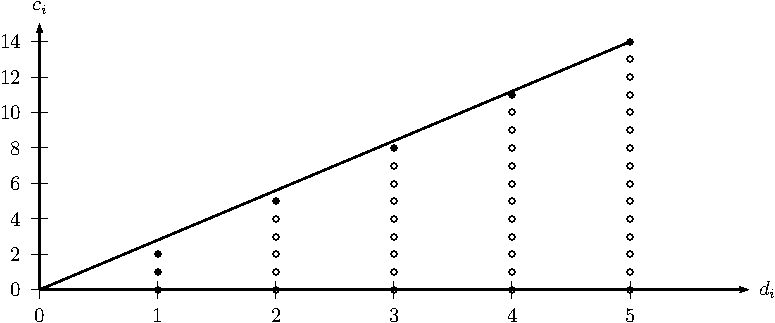
\includegraphics{pics/spin-lower-approximations-pic-pics.pdf}
\caption{This figure shows each non-negative best lower approximation of $\frac{14}{5}$ with a ``$\bullet$'' and each other lattice point below $5y=14x$ with a ``$\circ$''.  Note that the non-negative best lower approximations generate the monoid of lattice points in the first quadrant satisfying  $5y \le 14x$, with the operation $(a_1, b_1)(a_2, b_2)\mapsto (a_1 + a_2, b_1 + b_2)$ .}
\end{figure}

We can now prove our first adding-points lemma.

\begin{lem}
\label{lem:sat-1}
Let $X$ be a genus $g$ curve and $\halfcan' \in \di X \otimes \BQ$
satisfying $h^0(X, \lfloor{\halfcan'}\rfloor)\ge 1$. Suppose $P$ is not a base-point of $d\halfcan'$ for all $d\in \mathbb{N}$, meaning we can choose generators $u, x_1, \ldots, x_m$ of $R_{\halfcan'}$ in degree at most $\tau$ for some $\tau\in \mathbb{N}$, with $\deg u = 1$, $\ord_P^{\halfcan'}(x_i)=0$ for all $1 \leq i \leq m$, and $\ord_P^{\halfcan'}(u) = 0$.  Suppose $\halfcan = \halfcan' + \frac{\alpha}{\beta} P$
for some $\alpha,\beta \in \mathbb{N}$ such that
\begin{equation}
\label{eqn:deg1-sat-ind}
	h^0(X, \lfloor{d\halfcan}\rfloor) = h^0(X,\lfloor d\halfcan'
	\rfloor) + \left\lfloor d\frac{\alpha} {\beta} \right \rfloor \text{ for all } d \in \mathbb{
	N} \text{ such that } d \ge \frac{\beta}{\alpha},
\end{equation}
and let
\[
	0 < \frac{c_1}{d_1} < \ldots < \frac{c_n}{d_n} = \frac{\alpha}{\beta}
\]
be the positive best lower approximations of $\frac{\alpha}{\beta}$.
Then,

\begin{enumerate}
\item[(a)] $R_{\halfcan}$ is generated over $R_{\halfcan'}$ by elements $y_1, \ldots, y_n$ such that $\deg(y_i)=d_i$ and $-\ord_P^{L'}(y_i)=c_i$.

\item[(b)] Choose an ordering $\prec$ on $k[u, x_1, \ldots, x_m]$ such that
\[
	\ord_u(f) < \ord_u(g) \implies f\prec g.
\]
Equip $k[y_1, \ldots, y_n]$ with graded $P$-lex and $k[u, x_1, \ldots, x_m, y_1, \ldots, y_n]$ with the block order giving the order on $y_1, \ldots, y_n$ precedence over that on $u, x_1, \ldots, x_m$.  
If $I'$ and $I$ are the ideal of relations of $k[u, x_1, \ldots, x_m]\to R_{\halfcan'}$ and $k[u, x_1, \ldots, x_m, y_1, \ldots, y_n]\to R_{\halfcan}$ respectively, then 

\begin{align*}
	\initial_\prec(I) &= \initial_\prec(I') k[u, x_1, \ldots, x_m, y_1, \ldots, y_n] 
										 + \langle U_i: 1 \le i \le n-1 \rangle
										 + \langle V \rangle\\
\end{align*}
where 
$V=\{x_i y_j: 1\le i\le m, 1\le j\le n\}$
 and $U_i$ is the set of monomials of the form $\prod_{j=1}^{i} y_j^{a_j}$ with $a_j\in \mathbb{Z}^{\ge 0}$ such that
\begin{enumerate}
	\item[(1)] $\sum_{j=1}^i a_j c_j \ge c_{i+1}$\\
	\item[(2)] there does not exist $((b_1, \ldots b_i)\ne (a_1, \ldots a_i)$ with all $b_j\le a_j$ and $\sum_{j=1}^i b_jc_j\ge c_{i+1})$ \\
	\item[(3)] there does not exist $h<i$ such that $\sum_{j=1}^h y_j^{a_j}\ge c_{h+1}$
\end{enumerate}

\item[(c)] In particular, $R_\halfcan$ is generated over $R_\halfcan'$ in degrees at most $\beta$ with $I$ generated over $I'$ in degrees at most $\max(2\beta, \beta + \tau)$ (where $\tau = \max(1, \max_{1\le i, m}(\deg(x_i)))$.  \todo{Peter: Part (c) is immediate from (a) and (b), so maybe it shouldn't be its own section.  On the other hand, the other parts already have a lot of information written down (especial part (b)), so its not clear where it should be put.  Maybe in a remark after the lemma?}
%\item If $\gin_\prec(I')=\initial_\prec(I')$ then $\gin_\prec(I)=\initial_\prec(I)$.
%\item[(c)] A Gr\"{o}bner basis with the initial terms $y_i x_j$, $y_i y_j$,
%	and $(y_{\lfloor \frac{\alpha}{\beta} \rfloor})^{y_{\lfloor
%	\frac{\alpha}{\beta} \rfloor} + 1}$ (really the subset of these with positive subscripts) as shown above minimally
%generates $I'$.
\end{enumerate}
\end{lem}
\begin{proof}
By
Equation ~\ref{eqn:deg1-sat-ind}, for any $d
\in \mathbb{N}$ such that $\lfloor d \frac{ \alpha}{\beta} \rfloor > 0$,

\[
	h^0 (X, d \halfcan ) = h^0(X, d\halfcan') + \lfloor d\frac{\alpha}{\beta}\rfloor
\]

\noindent
so in $H^0 (X, \lfloor d\halfcan \rfloor)$ we can find elements with pole
order $i$ at $P$ for any $i \in \{0, \ldots, \lfloor d \frac{\alpha}{
\beta} \rfloor \}$. We will the use positive best lower approximations to
construct the generators $y_1, \ldots, y_n$ as described in the lemma's statement.

Let 
\[
	0 < \frac{c_1}{d_1} < \ldots < \frac{c_n}{d_n} = \frac{\alpha}{
	\beta}
\]

\noindent
be the positive best lower approximations of $\frac{
\alpha}{\beta}$. Note that a set of $\lfloor d_i \frac{\alpha}{\beta}\rfloor$ elements in $(R_{\halfcan})_{d_i}$ with respective pole orders $1, \ldots, \lfloor
d_i \frac{\alpha}{\beta} \rfloor$ (viewed as sections of $\so_{L'}$) are linearly independent over $(R_{\halfcan'})_d$, and thus by a dimension count form a $k$-basis for
$(R_{\halfcan})_d$ over $(R_{\halfcan'})_d$.

%For any $1\le i < j \le n$, we have $\frac{c_i}{d_i} < \frac{c_j}{d_j}$.  
Choose a positive best lower approximation $\frac{c_i}{d_i}$.  Let $z_1, \ldots, z_r \in R_\halfcan$ with $\sum_{j=1}^r \deg(z_j) = d_i$ and $\deg(z_j)<d_i$ for all $j\in \{1, \ldots r\}$.  Then for each $z_j$,
\[
	\frac{-\ord_P^{\halfcan'}(z_j)}{\deg(z_j)} < \frac{c_i}{d_i},
\]

\noindent
so
\[
	-\ord^{\halfcan'}_P(\prod_{j=1}^n z_j) = \sum_{j=1}^n -\ord^{\halfcan'}_P(z_j) < c_i .
\]

\noindent
Thus, the elements of $(R_{\halfcan})_{d_i}$ with pole order $c_i$ at $P$ are not generated by 
lower degrees. 
Choose some $y_i \in(R_{
\halfcan})_{d_i}$ with $-\ord_{P}^{L'}(y_i)=c_i$.  Note that this choice is generic if $d_i>1$ or $d_i=1$ and $c_i=\lfloor \frac{\alpha}{\beta}\rfloor$. 

Suppose $c,d\in \mathbb{N}$ with $d\le \beta$ and $\frac{c}{d} < \frac{\alpha}{
\beta}$ is not a best lower approximation.  Choose a
best lower approximation $\frac{c_i}{d_i}$ with $c_i$ maximal such that $d_i< d$.  This implies $\frac{c_i}{d_i}\ge \frac{c}{d}$ so 
%  The argument goes $c_i d \ge c d_i$
% implies c_i \frac{d}{d_i} \ge c
% implies c_i + \frac{d-d_i}{d_i}c_i \ge c
% \implies c_i (d-d_i) \frac{c_i}{d_i}\ge c
% so since everything is an integer $c_i +\lfloor (d - d_i) \frac{c_i}{d_i}\rfloor \ge c$
% \implies the equation below:
\begin{equation}\label{eqn:c-from-lower-terms}
	c_i +\lfloor (d-d_i) \frac{\alpha}{\beta} \rfloor \ge c.
\end{equation}

Using this fact, we recursively define a $k$-basis for $R_\halfcan$ over $R_{\halfcan'}$.  Define 
\[
	S_0 = \{u^l : l\in \mathbb{Z}^{\ge 0}\}
\]
and for each $i \in \mathbb{N}$, if $c_j$ is the maximal element among of $c_1, \ldots c_n$ such that $c_j \le i$ (note that this always exists since $1=c_1\le i$), define
\[
	S_i = y_j S_{i-j}.
\]
Observe that this recursive definition ensures that $S_i$ contains only elements $z\in R_\halfcan$ satisfying $-\ord^{\halfcan'}_P(z)=i$.
Then define 
\[
	S = \cup_{i=1}^{\infty} S_i.
\]
Note that $S_0$ is not part of this union and in fact $S\cap S_0 = \emptyset$ by pole order considerations.

Applying Equation \ref{eqn:c-from-lower-terms}, we see that $S$ contains elements in degree $d\in \mathbb{N}$ with each pole order in $1 \ldots, \lfloor d\frac{\alpha}{\beta}\rfloor$, so by dimension counting, $S$ forms a $k$-basis for $R_\halfcan$ over $R_{\halfcan'}$, so we have proven part (a).

Define $U_i$ and $V$ as in the lemma's statement and define
\[
	T = (\bigcup_{i=1}^{n-1} U_i) \cup V.
\]

We check that $S$, $T$, and $\prec$ meet the hypothesis of Lemma \ref{lem:relations_from_generators_induction}.  We have already shown $S$ forms a $k$-basis for $R_\halfcan$ over $R_{\halfcan'}$ giving us condition \ref{lem:relations_from_generators_induction}(1).  Our choice of order for monomials in $k[y_1, \ldots, y_n]$ and block order for those in $k[u, x_1, \ldots, x_m, y_1, \ldots, y_n]$ implies that $T\succ S\succ k[u, x_1, \ldots, x_m]$ giving us condition \ref{lem:relations_from_generators_induction}(2).  

Now, suppose $f\in k[u, x_1, \ldots, x_m, y_1, \ldots, y_n]$ is a monomial not contained in $k[u, x_1, \ldots, x_m]$, meaning there is some $j$ such that $y_j|f$.  Further suppose $f\not\in \langle V \rangle$, meaning that for each $i\in \{1, \ldots m\}$, $x_iy_j\not |f$ so $x_i\not|f$.  Therefore, $f\in k[u, y_1, \ldots, y_n]$.  We note that $S$ generates $y_j (k[u,y_1, \ldots, y_n])$ as a $k$-algebra.  That is, all monomials of $k[u, x_1, \ldots, x_m, y_1, \ldots, y_n]$ are contained in
\[
	k[u, x_1, \ldots, x_m] \cup V \cup \{y_1, \ldots, y_n\} k[u, y_1, \ldots, y_n]. 
\]
\todo{is $\{y_1, \ldots, y_n\} k[u, y_1, \ldots, y_n]$ appropriate notation to mean all possible products between some $y_j\in \{y_1, \ldots, y_n\}$ and some element in $k[u, y_1, \ldots, y_n]$?}
Thus, we see that if $f\in k[u, y_1, \ldots, y_n]$, then $f=u^b \prod_{j=1}^l {y_j}^{a_j}\in S$ for some $1\le l\le n$, $b\in \mathbb{Z}_{\ge 0}$, and $a_j\in \mathbb{Z}_{\ge 0}$ for all $j$ with $a_l> 0$.  For $j\in \mathbb{N}$ with $l < j\le n$, assign $a_j=0$.  If $i\in \{1, \ldots, n\}$, then $y_i f$ is either in $S$ or there is some $h\in \mathbb{N}$ such that $i\le h\le \max(i,l)$ satisfying $\prod_{j=1}^h y_j^{a_j}\not\in S_{\sum_{j=1}^h c_j a_j}$ \todo{Peter: terrible subscripts...}, and for all $r<h$, we have $\prod_{j=1}^r {y_j}^{a_j}\in S_{\sum_{j=1}^r c_ja_j}$.  We see that this latter case when $y_if\not\in S$ is equivalent to $\prod_{j=1}^h {y_j}^{a_j}\in U_h$.  Thus, since $S$ generates $\{y_1, \ldots, y_n\} k[y_1, \ldots, y_n]$ and $\bigcup_{i=1}^{n-1} U_i$ generates every monomial in $\{y_1, \ldots, y_n\} k[y_1, \ldots, y_n]-S$, we have shown that all monomials of $k[u, x_1, \ldots, x_m, y_1, \ldots, y_n]$ are contained in
\begin{align*}
				& k[u, x_1, \ldots, x_m] \cup \langle V \rangle \cup S \cup \langle \bigcup_{i=1}^{n-1} U_i \rangle \\
	\subseteq \; 	& S \cup \langle T\rangle \cup \initial_\prec(I') k[u, x_1, \ldots, x_m, y_1, \ldots, y_n] \; \cup \; k[u, x_1, \ldots, x_m].
\end{align*}
This gives us condition \ref{lem:relations_from_generators_induction}(3).  Thus, the conditions of Lemma \ref{lem:relations_from_generators_induction} are met, and by applying its conclusion we prove (b) of this lemma.  \todo{Peter: Checking that all the conditions of Lemma \ref{lem:relations_from_generators_induction}(2) are met takes a lot of space and clutter.  On the other hand, it is somewhat important.  Should it be included?}

Finally, (c) of this lemma follows immediately by looking at the constructions of parts (a) and (b).  






%Thus, for a general $d$ (not necessarily less than $\beta$), if $\frac{c}{d} \le
%\frac{\alpha}{\beta}$ is not a best lower approximation than we can
%construct an element in degree $d$ with pole degree $c$ by either $y
%_n^a y_i u^b$, $y_n^a zy_iu^b$ or $y_n^a z u^b$ satisfying the
%same conditions.  This forms a $k$-basis for $R_{\halfcan}$ over $R_{\halfcan'}$ and $y_1, \ldots, y_n$ generate $R_{\halfcan}$ over $R_{\halfcan'}$.  In particular, we see this generating set corresponds to the best positive approximations of $\frac{\alpha}{\beta}$.
%
%Choose $x_i\in \{x_1, \ldots, x_m\}$ and $y_j\in \{y_1, \ldots, y_n\}$.  Choose an element of the form $y_n^a y_l u^b$ and $y_n^a y_l y_{l'} u^b$ as described in the previous paragraph, in degree with $d_l= 1$ and if 
%$d_{l'}= 1$ then $c_{l'} = \lfloor \frac{\alpha}{\beta} \rfloor$. Specifically, we can 
%successively subtract some $\gamma_l y_l u^{b_l}$, $\gamma_l y_l z_l u^{b_l}$, or $
%\gamma_l z_l$ with $y_l, z_l, b_l$ satisfying the same conditions as above and $\gamma_l
%\in k$ the element ensuring that the difference decreases in pole degree at $P$ by 1. For 
%convenience, we can combine these into the case $\gamma_l (y_l)^{s_l}(z_l)^{a_l}u^{b_l}$ 
%with $(s_l,a_l)\in \{(1,0),(1,1),(0,1)\}$. In the cases when $\frac{\alpha}{\beta}<1$ so $z_l$ 
%is not well-defined, just pick an arbitrary element of $R_{\halfcan'}$ for $z_l$ ensuring that the 
%expression still makes sense; in such cases we will always choose $a_l= 0$ so this choice 
%is irrelevant, and only makes writing out cases more convenient. Therefore, we can write
%\[
	%x_i y_j - \sum_{l} (y_l)^{s_l} (z_l)^{a_l} u^{b_l}\in R_D
%\]
%
%\noindent
%giving us a non-trivial relation with leading term $x_i y_j$. \todo{Explicitly state ordering at 
%the beginning}
%
%Similarly, suppose $y_i, y_j\in \{y_1, \ldots , y_{n - 1}\}$ with $1
%< d_i$ and $j \ge i$ (that is, so $y_i y_j$ does not appear as a
%basis element of the form described above: $y_n^0 y_j y_i u^0$). 
%Choose the maximal $l$ such that $c_h \le c_i + c_j$; since $1 < d_i
%\le d_j$, $(c_i + c_j) - c_j>\lfloor \frac{\alpha}{\beta}\rfloor$
%so $c_{j + 1} < c_i + c_j$ meaning $c_h \ge c_{j + 1} > c_j$.
%Furthermore, $c_i + c_j - c_h < \lfloor \frac{\alpha}{\beta} \rfloor
%$ so either $c_h = c_i + c_j$ or there is some $h'$ such that $c_{h'}
%= c_i + c_j - c_l$ and $d_{h'}= 1$. Since $\frac{c_h}{d_h}$ is a
%best lower approximation of $\frac{\alpha}{\beta}$ with denominator
%larger than those of $\frac{c_i}{d_i}$ and $\frac{c_j}{d_j}$, we
%know that since $c_h\le c_i + c_j$ we must have $d_h < d_i + d_j$. 
%Thus in the case with a $y_{l'}$ term we have $d_h + d_{h'} = d_h +
%1 \le d_i + d_j$. That is to say, by choosing $b - d_i + d_j - a d_
%h - 1$ we find (where $a \in \{0,1\}$ corresponding to if a $y_{h'}$
%appears) that $y_h (y_h')^a u^b$ and $y_i y_j$ both lie in degree
%$d_i + d_j$ with pole order $c_i + c_j$ at $P$. From here we can
%follow a similar technique as in the previous paragraph to cancel
%out poles of $y_i y_j$ at $P $ to find
%\[
	%y_i y_j -\gamma_h (y_h)^{s_h}(z_{h})^{a_h}u^{b_h} -\sum_l (y_l)^{s_l} (z_{l})^{a_l}
	%u^{b_l}\in R_D
%\]
%
%\noindent
%implying a relation with initial term $y_i y_j$. 
%
%Next, suppose $y_i, y_j \in \{y_1, \ldots , y_{n - 1}\}$ such that
%$i \le j$, $d_j = d_i = 1$, and $d_{j + 1} = 1$ (i.e. $c_i, c_j \le
%\lfloor \frac{\alpha}{\beta} - 1 \rfloor$). If $i > 1$ and then $y_
%{j + 1} y_{i - 1}$ lies in the same degree as $y_i y_j$ (degree 2)
%with the same pole order; following the same method as the previous
%two paragraphs we find
%\[
	%y_i y_j - \gamma y_{i - 1} y_{j + 1} - \sum_{l} (y_l)^{s_l} (z_l)^{a_l}u^{b_l}\in R_D.
%\]
%
%\noindent
%Similarly if $i = 1$, then we get the same result using
%\[
	%y_i y_j - \gamma u y_{j + 1} - \sum_l y_l u^{b_l} \in R_D.
%\]
%
%\noindent
%In both cases we deduce that $y_i y_j$ is an initial term of some relation.
%
%
%Finally, we examine the case (for $\alpha \ge \beta$) of $(y_i)^{i +
%1}$ when $i = \lfloor \frac{\alpha}{\beta}\rfloor$. If $\beta = 1$,
%then there are no relations with initial term a power of $y_i$
%and we are immediately done. Otherwise, assuming $\beta \ne 1$, we
%note that $c_i d_{i + 1} = c_{i + 1} d_i + 1 = c_{i + 1} + 1$. \todo
%{reference to Evan's paper where he proves this} Therefore, if $i >
 %1$ then $c_i^{d_{i + 1} + 1}$ and $c_{i - 1} c_{i + 1}$ both lie
%in the $d_{i + 1} + 1$ degree with pole order $c_{i + 1} + 1$.
%Following a similar technique to the previous paragraphs we find
%\[
	%(y_i)^{c_{i + 1} + 1} - y_{i + 1} y_{i - 1} - \sum_l (y_l)^{s_l}(z_l)^{a_l} u^{b_l}.
%\]
%
%\noindent
%Similarly if $i = 1$ then
%\[
	%(y_i)^{c_{i + 1} + 1} - y_{i + 1}u - \sum_l (z_l)^{a_l} u^{b_l}.
%\]
%
%\noindent
%In each case we demonstrate $(y_i)^{c_{i + 1} + 1}$ as the initial term of a relation. 
%
%Let $J$ be the ideal of $k[u, x_1, \ldots, x_m, y_1, \ldots, y_n]$
%generated by the initial terms described in the previous paragraphs
%together with $\initial_\prec(I) k[u, x_1, \ldots, x_m, y_1, \ldots, y_n]$.
%
%We show that $J$ is in fact all of the initial ideal. Suppose
%$f$ is a non-constant monomial that does not lie within $J$.
%Further suppose $f$ does not lie in $k[u, x_1, \ldots, x_m]$. Then
%there is some $y_i \mid f$. Since $f \not\in j$, we cannot have
%some $x_j \mid f$ or else we would have $y_i x_j \mid f$
%contradicting $f \not\in J$. Furthermore, if $y_l \mid f$ for $l <
%i$, then we must have $d_l = 1$ or else $y_l y_i$ is an initial
%element of a relation and divides $f$. If $d_i = 1$ as well, then
%we must have $c_i = \lfloor \frac{\alpha} {\beta} \rfloor$, or else
%$y_i y_l \in I$; finally we can not have $(y_{\lfloor \frac{\alpha}{
%\beta} \rfloor})^{d_{\lfloor \frac{\alpha}{\beta} \rfloor + 1} + 1} \mid
%f$. We observe that the remaining elements are precisely those of
%the form $y_n^a y_i u^b$, $y_n^a z y_i u^b$, and $y_n^a z u^b$
%which are the elements of our chosen $k$-basis for $k[u, x_1, \ldots
%, x_m, y_1, \ldots, y_n]/I'$ over $k[u, x_1, \ldots, x_m]/I$.
%Therefore, by dimension counting (in each degree), we see that $J$
%is the initial ideal of $I$. 


%Furthermore, since our choice of $y_i
%$'s was generic, this is in fact the generic initial ideal.

%In the case when all $\frac{\alpha}{\beta}\le 1$, Lemma
%~\ref{lem:minimal_quadratic} immediately tells us that the Gr\"{o}bner
%basis defined above is minimal.
%\todo{What about $\frac{\alpha}{\beta} > 1$?}
\end{proof}

\begin{rem}\label{rem:quad-gen}
If $\frac{\alpha}{\beta}=\frac{e_i-1}{2 e_i P_i}$ for some odd $3\le e_i\in \mathbb{N}$, then $T$ from Lemma \ref{lem:sat-1} consists only of terms of the form $x_i y_j$ and $y_i y_j$, which are quadratic in the generators.
\end{rem}


\begin{rem}\label{rem:sat-1-gen-lem-generic}
The generators in Lemma \ref{lem:sat-1} are generic if $\frac{\alpha}{\beta}\le 1$ (since there is at most one positive best lower approximation $\frac{c_i}{d_i}$ with $d_i=1$).  When $\frac{\alpha}{\beta}>1$, the choice of generators in degrees great than 1 is generic; furthermore, we can make the choice in degree 1 generic by choosing $\lfloor \frac{\alpha}{\beta}\rfloor$ linearly independent elements in degree 1 with pole at $P$ of order $\lfloor \frac{\alpha}{\beta}\rfloor$ rather than elements with poles of order $1, \ldots, \lfloor \frac{\alpha}{\beta}\rfloor$; this requires minor complications in the construction of generators of the ideal of relations.
\end{rem}

We now restrict our attention to log canonical rings of stacky curves.  Lemma \ref{lem:sat-1} accounts for the relevant induction cases when the spin canonical ring is already saturated in 1.  We complement it with the following two lemmas that allow us to inductively add points, under certain conditions when the spin canonical ring is saturated at degrees two and three.

\begin{lem}
\label{lem:sat-2}
Let $(\sx, \Delta, \halfcan_\sx)$ and $(\sx', \Delta, \halfcan_{\sx'})$ be log spin curves with coarse space $(X, \Delta, \halfcan_X)$ having signatures $(g; e_1, \ldots, e_r; \delta)$ and $(g, e_1, \ldots, e_{r- 1}, \delta)$, where $e_r=3$.  Suppose $g > 0,$ and, if $g = 1$ then $\deg 3\halfcan' \geq 2$ (note that this implies $\sat(Eff(L'))\le 2$).
Let $R_{L'} = k[x_2, x_3
, x_5, \ldots, x_m]/I'$ and let $\halfcan = \halfcan' + \frac{1}{
3}P$, where $P\in X$ is a base point of $\halfcan'$ (which includes the case when $H^0(X, \lfloor \halfcan'\rfloor) = 0$).
Suppose for $i \in \{2, 3\}$, $\deg x_i = i$ and $\ord_P^{\halfcan'}(x_i)= 0$ (which is satisfied generically in degree 2 and 3, since base-point freeness follows by Riemann-Roch). Choose an ordering on $k[x_2, \ldots, x_m]$ that satisfies
\begin{align*}
	\ord_{x_2}(f) < \ord_{x_2}(g) \implies f \prec g.
\end{align*}

\noindent
Then, the following statements hold.

\begin{enumerate}
	\item[(a)] General elements  $y_i \in H^0(\sx,iL)$ for $i \in
		\{3, 4\}$ satisfy $-\ord_P^{\halfcan'}(y_i) = 1$ and any such choice of elements
		$y_3, y_4,$ minimally generate $R$ over $R'$.
	\item[(b)] Equip $k[y_3, y_4]$ with $grevlex$ so that $y_3 \prec 
		y_4$
		and equip the ring $k[y_3, y_4, x]$ with the block 
		order with $x_2, \ldots, x_m$ preceding $y_3, y_4$.  Then
		\begin{align*}
			\initial_\prec(I) &= \initial_\prec(I')k[x, y_3, y_4]+\langle y_4 x_j \mid 2 \leq j \leq m \rangle +\langle y_4^2 \rangle.
		\end{align*}
	%\item[(c)] Any set of minimal generators for $I'$ together with 
		%any set of relations with leading terms as in (b) minimally 
		%generate $I$.
\end{enumerate}
\end{lem}

\begin{proof}
The assumptions on $g$ imply $H^0(\sx, 3L), H^0(\sx, 4L)$ are both base point free: If $g \geq 2$ then $\deg 3L > 2g - 1$ and $\deg 4L > 2g - 1$, so $H^0(\sx, 3L)$ and $H^0(\sx, 4L)$ are base point free. If $g = 1$, we assume $\deg 3L \geq 2 > 2g - 1$, so we also have $\deg 4L \geq 2 > 2g - 1,$ so again $H^0(\sx, 3L)$ and $H^0(\sx, 4L)$ are base point free. Therefore, general elements $y_3$ and $y_4$ satisfy $-\ord_P^{\halfcan'}(y_i) = 1$ by Riemann-Roch. \todo{Understand why/whether we need to cite Lemma 5.4.7.} 

A quick computation checks that
the following is a $k$ basis for $R$ over $R'$:

\begin{align}
\label{eqn:sat_two_add_generator}
	S =	& \; \{ y_3^ax_2^b x_3^\epsilon \mid a \geq 0, b 
		\geq 0, \epsilon \in \{0, 1\}\} \cup \{ y_3^ay_4 \mid a \geq 0 \}
\end{align}

\noindent
completing part (a).

Letting
\begin{align*}
	T =   &\; \{ y_4 x_j \mid 2 \leq j \leq m \}\cup \{ y_4^2 \}
\end{align*}
a similar (but much easier) computation to that of lemma $\ref{lem:sat-1}$ determines that $S$, $T$, and $\prec$ meet the conditions of Lemma \ref{lem:relations_from_generators_induction}, whose result then immediately implies part (b).


%For any $x_j$, notice that $-\ord_P(y_4x_j)\le 1$. If it is non-positive, then it lies in $R_{\halfcan'}$ immediately giving us a relation with initial term $y_4x_j$. Otherwise, 
%we can choose $A_j \in k$ and $w_j\in R_{\halfcan'}$ such that $y_4x_j -A_jy_3w_j$ has no pole at $P$ and thus lies in $R_{\halfcan'}$ giving us a desired relation. 
%Similarly, we can find $B, C \in k$ such that $y_4^2 + B y_3^2 x_2+ Cy_3x_2x_3$ has no pole at $P$ and is thus in $R_D$. In both cases we induce a relation, with initial term described in the lemma's statement. Noting that any monomial is either a multiple of one of these initial terms, is a basis element (described above), or is in $R_D$, we see that these monomials in fact generate the initial ideal of $I$ over $\initial(I')$.
%Finally, (c) follows immediately from Lemma ~\ref{lem:minimal_quadratic}.

\end{proof}

\begin{lem}
\label{lem:sat-3}
\todo{Make explicit assumptions on genus.}
Suppose $L'$ is a log half-canonical divisor of $\sx'$ with coarse
space $X$ of genus 0 such that $\sat(\Eff(\halfcan')) = 3$ and $R_
{\halfcan'} = k[x_3, x_4 , x_5, \ldots, x_m]/I'$; since we are in genus 0, we can choose $x_3, \ldots, x_m$ such that $-\ord^{L'}_P(x_i)=0$ for all $i$. Let $L = L' + \frac
{1}{3}P$. Suppose $\deg x_i = i$ for $i \in \{3, 4, 5\}$ and that
the ordering on $k[x_3, \ldots, x_m]$ satisfies
\begin{align*}
	\ord_{x_3}(f) < \ord_{x_3}(h) \implies f \prec h.
\end{align*}

\noindent
Then, the following statements hold.

\begin{enumerate}
	\item[(a)] General elements  $y_i \in H^0(\sx, iL)$ for $i \in \{3,
		4,5\}$ satisfy $-\ord_P^{\halfcan'}(y_i) = 1$ and any such choice of elements $y
		_3, y_4,$ and $y_5$ minimally generate $R$ over $R'$.
	\item[(b)] Equip $k[y_3, y_4, y_5]$ with $grevlex$ so that $y_3 \prec 
		y_4 \prec y_5$
		and equip the ring $k[y_3, y_4, y_5, x]$ with the block order so that $x_3, \ldots, x_m$ precede $y_3, y_4, y_5$.  Then,
		\begin{align*}
			\initial_\prec(I) &= \initial_\prec(I) k[x, y_3, y_4, y_5] \\
			&+ \langle y_i x_j \mid 4 \leq i \leq 5, 3 \leq j \leq m\rangle \\
			&+ \langle y_i y_k \mid 4 \leq i \leq j \leq 5\rangle.
		\end{align*}
	%\item[(c)] Any set of generators for $I'$ together with 
	%	any set of relations with leading terms as in (b) 
	%	generate $I$.
\end{enumerate}
\end{lem}

\begin{proof}
Since we are in genus 0, general
elements $y_3, y_4,$ and $y_5$ in weights 3, 4, and 5 respectively satisfy $- \ord_P^{\halfcan'}(y_i) =
1$. \todo{Understand why/whether we need to cite 
Lemma 5.4.7.  Peter: What does this mean?}  We see by pole order considerations that

\begin{align}
\label{eqn:add_one_generator}
	\begin{split}
	S=	&\{ y_3^ax_3^b x_4^\epsilon x_5^{\epsilon'} \mid a \geq 0, b 
		\geq 0,(\epsilon,\epsilon') \in \{(0,0),(0,1),(1,0)\} \} \\
	\cup \;&\{y_3^ay_4, y_3^by_5 \mid a \geq 0, b \geq 0 \}
	\end{split}
\end{align}

\noindent forms a $k$ basis for $R$ over $R'$, which concludes part (a) of the proof.

Setting
\[
	T = \{ y_i x_j \mid 4 \leq i \leq 5, 3 \leq j \leq m\}+ \{ y_i y_k \mid 4 \leq i \leq j \leq 5\} 
\]
we can argue similarly to Lemma $\ref{lem:sat-1}$ that $S$ and $T$ along with $\prec$ satisfy the hypothesis of Lemma \ref{lem:relations_from_generators_induction}, immediately implying part (b) of this proof.



%To see these generate $R'$ over $R$, note that $\dim_k R'_d - \dim_k R
%_d = \lfloor \frac{d}{3} \rfloor,$ by Riemann--Roch. So, it
%suffices to show that we have precisely $\lfloor \frac{d}{3} \rfloor
%,$ elements of degree $d$ in the claimed basis of
%~\ref{eqn:add_one_generator}. Indeed, letting $a = \lfloor \frac{d}{3}
%\rfloor $ and $b = d \bmod 3$, we have that the elements
%
%\begin{align*}
	%x_3^{a- 1}x_{3+b}, y_3x_3^{a-2}x_{3+b}, \ldots, y_3^ax_{3+b}, y_3^ay_{
%3+b}
%\end{align*}
%
%\noindent
%are precisely $a$ elements, which are all independent as they have
%distinct pole orders at $P$. This completes part (a).
%
%To show part (b), note that the generators in
%~\ref{eqn:add_one_generator} are precisely a set of monomials which
%generate $k[x, y]/J$ over $k$. So, to show $J = in_\prec(I)$, it
%suffices to show that all generators of $J$ lie in $in_\prec(I)$.
%
%This follows, since there exist constants $A_{i,j} \in k$ for $4
%\leq i \leq 5,3 \leq j \leq m,$ elements $B_1,B_2,B_3 \in k$ and
%elements $w_{i,j} \in R'$ so that the following linear combinations
%of elements lie in $R'$.
%
%\begin{align*}
	%&y_i x_j - A_{i,j} y_{i - 1}w_j \text{ so that } 4 \leq i \leq 5,3
	%\leq j \leq m \text{ and } \deg w_j = \deg x_j + 1 \\
	%&y_4^2 + B_1 y_3 y_5 \\
	%&y_4 y_5 + B_2 y_3^2 x_3 \\
	%&y_5^2 + B_3 y_3^2 x_4
%\end{align*}
%
%\noindent
%Of course, the initial terms of these elements are precisely the
%generators of $J$, completing (b).


%Finally, (c) follows immediately from Lemma ~\ref{lem:minimal_quadratic}
\end{proof}


%\begin{lem}
%\label{lem:adding_points_saturation_2_to_1_with_log}
%Let $(\sx, \Delta, \halfcan)$ and $(\sx, \Delta', L')$ be log spin log stacky spin 
%curves with $0\ne \Delta=\Delta'+2P$ for some non-stacky point $P$ not in the support of $
%\halfcan'$, meaning that $L=L'+P$. Let $(g; e_1, \ldots, e_\tau; \delta+2)$ and $(g; e_1, 
%\ldots, e_\tau, \delta)$ with $g\ge 2$ be their respective signatures. Suppose 
%$\sat(\Eff(\halfcan))= 1$ and $\sat(\Eff(\halfcan'))=2$. Further suppose $R_{\halfcan'} = k[x_2, 
%x_3, \ldots, x_m]/I'$ with $\deg(x_2) = 2$ and $\deg(x_3) = 3$. Then
%
%\begin{enumerate}
%\item[(a)] Then generic elements $y_1$ and $y_2$ in $(R_{\halfcan})_1$ and $
%(R_{\halfcan})_2$ respectively, such that $-\ord_P(y_2)> 0$ and $\{y_1^2, y_2\}$ is linearly 
%independent, generate $R_\halfcan$ over $R_{\halfcan'}$.
%\item[(b)] Equip $k[y_1, y_2]$ with $grlex$ so that $y_2 \prec y_1$ and equip $k[y_1, y_2, 
%x_2, \ldots, x_m]$ with the block order so that $R_\halfcan=k[y_1, y_2, x_2, \ldots, x_m]/I$. 
%Then
%\begin{align*}
			%in_\prec(I) &= in_\prec(I')k[x_2, \ldots, x_m, y_1, y_2] \\
			%&+\langle y_2 x_j \mid 2 \leq j \leq m \rangle \\
			%&+\langle y_2^2\rangle.
		%\end{align*}
%\item[(c)] Any set of minimal generators for $I'$ together with any set of relations with 
%leading terms as above minimally generate $I$.
%\end{enumerate}
%\end{lem}
%
%\begin{proof}
%Since adding $P$ to $L'$, reduces saturation from 2 to 1, $h^0(X, \lfloor L \rfloor)= 1$. 
%Choose any $y_1\in H^0(X,\lfloor L\rfloor)$; we know by saturation arguments that $-
%\ord_P(y_1)= 1$. Furthermore, since $\delta> 0$, we use Riemann-Roch to deduce that for 
%all $d> 1$ $h^0(X,\lfloor dL\rfloor)=h^0(dL') +d$, so $(R_\halfcan)_d$ is a $d$ dimension $k
%$-vector space over $(R_{\halfcan'})_d$. In particular, this means we can generically 
%choose an element $y_2\in H^0(X,\lfloor 2L\rfloor)$ linearly independent from $y_1^2$. By 
%dimension counting, we see that 
%\[
	%\langle y_1^a x_2^b x_3^c: a\ge 0, b\ge 0, c\in \{0,1\}\rangle
%\]
%\[
	%\langle y_1^a y_2: a\ge 0\rangle
%\]
%form a $k$-basis for $R_\halfcan$ over $R_{\halfcan'}$. This completes part (a).
%
%To show part (b), we note that the monomials in the basis above generate $k[x, y]/\initial_
%\prec(I)$. Thus, it is sufficient to show that $J\subseteq \initial_\prec(I)$. For $j\ge 2$, we 
%can choose $w_j$ in degree $\deg(x_j) + 1$ and $A_j\in k$ such that
%\[
	%y_2x_j -A_jy_3w_j
%\]
%has no pole at $P$ at thus lies in $R_{\halfcan'}$. Similarly, we can choose $B$ and $C$ 
%such that
%\[y^2_4+By_1^2x_2+Cy_1x_3\]
%has no pole at $P$, so it lies in $R_{\halfcan'}$. These give us relations with initial terms 
%as desired, concluding part (b).
%
%Finally, (c) follows immediately from Lemma ~\ref{lem:minimal_quadratic}.
%
%\end{proof}
%
%\begin{lem}
%\label{lem:adding_points_saturation_2_to_1_no_log}
%Let $(\sx, 2P, \halfcan)$ and $(\sx, 0, L')$ be log spin log stacky spin curves 
%with $P$ not in the support of $\halfcan'$, meaning that $L=L'+P$. Let $(g; e_1, \ldots, e_
%\tau; 2)$ and $(g; e_1, \ldots, e_\tau, 0)$ with $g\ge 2$ be their respective signatures. 
%Suppose $'\sat(\Eff(\halfcan))= 1$ and $'\sat(\Eff(\halfcan'))=2$. Further suppose 
%$R_{\halfcan'} = k[x_2, x_3, \ldots, x_m]/I'$ with $\deg(x_2) = 2$ and $\deg(x_3) = 3$. 
%Then
%\begin{enumerate}
%\item[(a)] Then generic elements $y_1$ and $y_3$ in $(R_{\halfcan})_1$ and $
%(R_{\halfcan})_3$ respectively, such that $-\ord_P(y_3)> 1$ and $\{y_1^3, y_2\}$ is linearly 
%independent, generate $R_\halfcan$ over $R_{\halfcan'}$.
%\item[(b)] Equip $k[y_1, y_3]$ with $grlex$ so that $y_3 \prec y_1$ and equip $k[y_1, y_3, 
%x_2, \ldots, x_m]$ with the block order so that $R_\halfcan=k[y_1, y_3, x_2, \ldots, x_m]/I$. 
%Then
%\begin{align*}
			%in_\prec(I) &= in_\prec(I')k[x_2, \ldots, x_m, y_1, y_2] \\
			%&+\langle y_3 x_j \mid 2 \leq j \leq m \rangle \\
			%&+\langle y_3^2
		%\end{align*}
%\item[(c)] Any set of minimal generators for $I'$ together with any set of relations with 
%leading terms as above minimally generate $I$.
%\end{enumerate}
%\end{lem}
%\begin{proof}
%The proof follows similarly to that of Lemma 
%\ref{lem:adding_points_saturation_2_to_1_with_log}, with the change that $(R_
%\halfcan)_2$ is only a degree 1 $k$-vector space over $(R_{\halfcan'})_2$ forcing a 
%generator in degree 3 rather than degree 2. 
%\end{proof}
%
%We prove an inductive theorem on adding 2-sat here.
%
%
%We will now prove a Lemma that will be used to inductively deal with divisors that are sufficiently saturated, by combining and extending methods of VZB \todo{add 
%reference} and O'Dorney\todo{reference}.
%
%\begin{rem}\label{rem:deg1_sat_ind_gen_rel_degrees}
%Notice that in Lemma ~\ref{lem:deg1_sat_ind}, $D'$ is generated in degree at most $\max(\bar{d}, \beta)$ with relations generated in degree at most $\max(\bar{\tau}, \bar{d} + \beta, 2 \beta)$
%\end{rem}
%
%This yields some immediate corollaries:
%
%\begin{cor}\label{cor:effective_Q_divisor_can_ring}
%If the genus of $X$ is 0 and $D\sim\sum \frac{\alpha_i}{\beta_i} P_i$ is linearly equivalent to an effective $\BQ$ divisor of $X$, then $R_D$ is generated in degree at most $\max(\beta_i,1)$ with relations generated in degree at most $2\max(\beta_i,1)$.
%\end{cor}
%
%\begin{proof}
%We can prove this by induction. As a base case, let $D\sim 0$. Then $R_D\cong k[x]$ which is generated in degree 1 with no relations, satisfying the inductive hypothesis.
%Now, suppose the result is proven for all effective $D$ with support at most $r$ points; then if $D'\sim \sum_{i = 1}^{r+ 1} \frac{\alpha_i}{\beta_i}$, we set $D=\sum_i^{r} \frac{\alpha_i}{\beta_i}$. By hypothesis, $R_D$ is generated in degree at most $\max_{1\le i\le r}(\beta_i)$ with relations generated in degree at most 2$\max_{1\le i\le r}(\beta_i)$. Since $D$ is effective, the condition of equation ~\ref{eqn:deg1-sat-ind} is met, so by remark ~\ref{rem:deg1_sat_ind_gen_rel_degrees} of Lemma ~\ref{lem:deg1_sat_ind}, $R_{D'}$ is generated in degree at most $\max(\beta_i)$ with relations generated in degree at most $2\max(\beta_i)$.
%\end{proof}
%
%\todo{do these corollaries fit here?}
%
%\begin{cor}\label{cor:genus_0_positive_delta}
%Let $\halfcan$ be a stacky log spin canonical divisor of $(X,\Delta)$ with signature $(g;e_1, \ldots, e_n;\delta)$ such that $2\halfcan=K_\sx+\Delta$ with $\delta=\deg(\Delta)> 0$. Then $\halfcan$ is effective so we can inductively apply Lemma ~\ref{lem:deg1_sat_ind}.
%\end{cor}
%\begin{proof}
%Since $\halfcan$ is a half canonical divisor, 
%\[
	%2\halfcan=D+\sum \subhalf{e_i}P_i
%\] 
%where 
%\[
	%D\sim K_X+\Delta\sim -2\infty+ \Delta
%\] is a divisor of $X$ (i.e. with 
%possibly negative integer coefficients). Since $\Delta$ is non-
%zero effective, $\deg(D)\ge - 1$.  Noting that the coefficient of 
%any point $P$ occurring in a stacky divisor of $\sx$ must have 
%coefficient lying in $\mathbb{Z}[\frac{1}{e_i}]$ (ranging over $e_i$
%s appearing in the characteristic of $(\sx,\Delta)$).
 %
%Since all $e_i$'s are odd, $2$ cannot appear in a denominator of the 
%coefficient of a point $P$ in $\halfcan$, meaning that $\frac{D}{2}$
 %must be a $X$-divisor. Since $\deg(\frac{D}{2})=\frac{1}{2}\deg(D)
%\ge -\frac{1}{2}$, we in fact have $\deg(D)\ge 0$. Thus $\halfcan$ 
%is linearly equivalent to an effective $X$ divisor plus $\sum 
%\subhalf{i}P_i$. We have thus shown $\halfcan$ is linearly equivalent to an effective divisor. Thus, by ~\ref{cor:effective_Q_divisor_can_ring} the desired result follows.
%\end{proof}

%\todo{Move this Lemma:}
%\begin{lem}\label{lem:add_point_effective_divisor_no_deg_1_generators}
%Let $(X,\Delta,\halfcan)\to (X,\Delta',\halfcan)$ be the natural map of genus $g$ log curves with $\Delta=\Delta'+P$, such that $2\halfcan\sim K_X+\Delta$, $2\halfcan'\sim K_X+\Delta'$, and $\Delta=\Delta'+P$ with $\Delta'\ne 0$ for some $P\not\in supp(\halfcan)$. 
%Suppose $\deg(\lfloor{\halfcan}\rfloor)=\deg(\lfloor \halfcan'\rfloor)\ge 0$, so $R_{\halfcan}$ has a
%generator $u$ in degree 1, and $R_{\halfcan'}$ has no new generators in degree 0. Suppose $D$ is generated by $u, x_1, \ldots, x_m$ in degree at most $\bar{d}$ with relations generated 
%in degree at most $\bar{\tau}$.
%Then 
%\begin{itemize}
%\item $R_{D'}$ is generated over $R_D$ by elements $y_1, y_2, y_3$ in degrees 2, 2, and 3 respectively. 
%\item If $I$ and $I'$ are the ideal of relations of $R_D$ and $R_{D'}$ respectively, then 
%
%\begin{align*}
	%\initial_\prec(I') &= \initial_\prec(I) k[u, x_1, \ldots, x_m, y_1, \ldots, y_n] \\
										 %&+ \langle y_i x_j \rangle \\
										 %&+ \langle y_3^2, y_3y_2, y_2y_1, y_1^2\rangle \\
%\end{align*}
%\item A Gr\"{o}bner basis with initial terms described above minimally generates $I'$ over $I$.
%\end{itemize}
%\end{lem}
%\begin{proof}
%Similar to all the other Lemmas\todo{combine sections?}
%\end{proof}

One can prove similar results in cases with different conditions on saturation, base-point freeness, and the coefficients of added points, but only these three cases (Lemmas ~\ref{lem:sat-1}, ~\ref{lem:sat-2}, and ~\ref{lem:sat-3}) are needed for the remainder of this paper.  Instead we turn now to inductive methods to incrementally increase the $e_i$s.  Combined with the adding points lemmas, these will provide all the necessary inductive tools for the remainder of the paper.

\ssec{Raising Stabilizer Orders}
\label{ssec:raise-orders}
In this subsection, we aim to prove Lemma
~\ref{lem:raise-stacky-order}, whose proof is almost identical to that of \cite[Theorem 8.5.7]{vzb:stacky}. In many cases, Lemma ~\ref{lem:raise-stacky-order} implies that if the main result, Theorem 
~\ref{thm:main}, holds for a curve with signature
$(g;e_1', \ldots, e_k', e_{k+1}' \ldots, e_r';\delta),$ with $e_{k+1}' = \cdots = e_r',$ then Theorem ~\ref{thm:main} also holds for a curve with
signature $(g; e_1', \ldots, e_k',e_{k+1}'+2,\ldots, e_r'+2; \delta).$ In order to state Lemma
~\ref{lem:raise-stacky-order}, we will need to define a certain notion of admissibility in Definition ~\ref{defn:admissible}, which is quite similar to \cite[Definition 8.5.1]{vzb:stacky}.

One key difference between the notion of admissibility in Definition ~\ref{defn:admissible} and \cite[Definition 8.5.1]{vzb:stacky} is that in \cite{vzb:stacky}, Voight and Zureick-Brown may assume that $\{P_i\} \cap \Supp(K_X) = \emptyset.$ However, we cannot assume that $\{P_i\} \cap \Supp(L_X) = \emptyset$, as $L_X$ is not necessarily basepoint-free. Therefore, we will have to work with orders of zeros of poles relative to the divisor we are inducting from, instead of relative to the structure sheaf.

\begin{defn}
\label{defn:admissible}
Let $(\sx', \Delta, L'),(\sx, \Delta , L)$ be log spin
curves, with the same stacky points $Q_1, \ldots, Q_r$. Let $J \subset
\{1, \ldots, r\}$. Suppose $e_i'+ 2 \chi_J (i) = e_i$ where

$$\chi_J(i) = \begin{cases}
	1, &\text{ if }i \in J\\
	0, &\text{ otherwise. } 
\end{cases}$$

Let $R'$ be the canonical ring associated to $\sx'$. Define $(\sx',L',J)$
to be {\bf admissible} if the $R'$ admits a presentation
\begin{align*}
	R' \cong \left( k[x_1, \ldots, x_m] \otimes k[y_{i, e_i'}]_{i \in J} \right)/I'
\end{align*}

\noindent
with $y_{i, e_i'} \in R'$ for each $i \in J$ such that the following
three conditions hold.


\todo{Peter:I'm still kind of unhappy with the notation $y_{e_i'}$ because it is treating $e_i'$ like a formal object rather than a number. What I mean is if $e_1'=e_2'$ that a reader might reasonably interpret $y_{e_1'}$ the same as $y_{e_2'}$. Aaron: By all means, please suggest better notation and we can discuss it. However, I think your particular concern is well answered because we include the further subscript $i$. That is, $y_{1,e_1} \neq y_{2,e_2}$ even if $e_1 = e_2=5$, because $y_{1,5}$ and $y_{2,5}$ are different variables. Another thing to note here is that $e_i' = e_i + 2,$ so that the two will never be equal. Does this assuage your concern? Also, Further, when I read David's paper, he used this notation, and I was never confused by this notation.}
\begin{enumerate}
	\item[(Ad-i)] First, 
	\begin{align*}
	\deg y_{e_i'} &= e_i'  &\text{ and } &&-\ord_{Q_i}^{\halfcan_X'}(y_{i, e_i'})
		= \frac{e_i'- 1}{2}.
	\end{align*}
		\item[(Ad-ii)] Second, every generator $z \neq y_{i, e_i'}$	of $R'$ satisfies
		\begin{align*}
			\frac{-\ord_{Q_i}
^{\halfcan_X'}(z)}{\deg z} < \subhalf {e_i'}.
		\end{align*}
	\item[(Ad-iii)] Third, we have
		\begin{align*}
			\deg \lfloor e_i L \rfloor \geq 2g - 1 + \max_{d \geq 0} \# S_{\sigma, J}(i, d)
		\end{align*}
		where
		\begin{align*}
			S_{\sigma, J}(i, d) := \{j \in J : j \neq i \text{ and } e_j'+2d
			\mid e_i - e_j'\}
		\end{align*}
\end{enumerate}
\end{defn}

\begin{rem}
Note that $S_{\sigma,J}(i,d-1)$ as defined in condition (Ad-iii) of Definition ~\ref{defn:admissible} can equivalently be defined as $S_{\sigma,J}(i,d-1)= \{j \in J : j \neq i \text{ and }(e_j' + 2d-2)|e_i' + 2d\}.$ Written this way, $\# S_{\sigma,J}(i,d-1)$ is more apparently similar to $\mu(i,d)$ as defined in \cite[Defintion 8.5.1]{vzb:stacky}.
\end{rem}


%\begin{lem}\label{lem:n-3s-admissible}
%Fix a genus $g$, a log divisor $\Delta$, and a coarse space $X$. Suppose $3\le r\in \BN$ so that all stacky curves $\sx'$ with $r- 1$ stacky points of degree 3 over the coarse space $X$ have all subsets $J'$ of $\{e_1, \ldots, e_{r- 1}\}$ admissible in $L'$. Then if $\sx$ has coarse space $X$, any subset of $J$ of $\{e_1, \ldots, e_r\}$ (with all $e_i =3$) is admissible viewed in $L$.
%\end{lem}
%\begin{proof}
%To show (Ad-i) and (Ad-ii) look at some $\sx'$ with $r- 1$ stacky points $'s=\{Q_1, \ldots, Q_{j - 1}, Q_{j + 1}, \ldots Q_r\}$ including a chosen $Q_i$ (and excluding some $Q_j\ne Q_i$). Then select $y_{e_r'}$ from the choice that makes the set $J'=\{i\}$ an admissible set in $\sx'$; this naturally can be seen inside of $R_{\sx}$ and satisfies (Ad-i). Furthermore, since $s$ is an admissible set of $L'$, in particular, we must have (Ad-ii) satisfied so $\frac{-\ord_{Q_l}
%^{\halfcan_X'}(y_i)}{\deg (y_i)} = 0$ for\todo{I'm confused how (Ad-ii) follows in genus 0?}
%
 %follows immediately from the base-point freeness of $3\halfcan$ which we have for the following reasons in the various genera:
%\begin{itemize}
%\item When $g> 0$, $\deg(\lfloor 3 L\rfloor)\ge 3g-3+2\ge 2g$ (the added two comes from the fact that $r\ge 2$).
%\item When $g= 0$, since $L'$ has a nontrivial admissible subset within $\{e_1, \ldots, e_{r- 1}\}$ satisfying (Ad-i), we know $\deg(\lfloor 3\lfloor)\ge 0$, so it is base-point free.
%\end{itemize}
%\end{proof}

The following Lemma will slightly strengthen condition (Ad-ii) from Definition ~\ref{defn:admissible} and this improvement is crucially used in the proof of part (c) of Lemma ~\ref{lem:raise-stacky-order}. Lemma ~\ref{lem:admissible_inequality} can be thought of as an analog of \cite[Lemma 8.5.3]{vzb:stacky}

\begin{lem}
\label{lem:admissible_inequality}
Condition (Ad-ii) of Definition ~\ref{defn:admissible} implies the
stronger condition that

\begin{align*}
	-\ord_{Q_i}
^{\halfcan_X'}(z) \leq \deg(z) \subhalf{e_i'} -\frac{1}{e_i'}
\end{align*}
\end{lem}

\begin{proof}
We know by (Ad-ii) that

\begin{align*}
	-\ord_{Q_i}
^{\halfcan_X'}(z) < \deg(z) \subhalf{e_i'}
\end{align*}

\noindent
If we write $\frac{\alpha}{\beta} = \deg(z) \frac{e_i'- 1}{2e_i'}$ 
as a fraction in lowest terms, then we see $\beta \mid e_i'$ since $
e_i'- 1$ is even. Therefore, since $-\ord_{Q_i}
^{\halfcan_X'}(z)$ is an integer, 
we must have

\begin{align*}
	-\ord_{Q_i}
^{\halfcan_X'}(z) \leq \deg(z) \subhalf{e_i'} - \frac{1}{\beta} \leq 
	\deg(z) \subhalf{e_i'} - \frac{1}{e_i'}.
\end{align*}
\end{proof}

\begin{lem}
\label{lem:admissible_subset}
If $(\sx',\Delta,L')$ is a log spin curve, $(\sx',L', J)$ is admissible and $W \subset J$ is any subset,
then $(\sx', L', W)$ is also admissible.
\end{lem}

\begin{proof}
Each of the conditions (Ad-i), (Ad-ii), and (Ad-iii) hold for $W$
if they hold for $J$.
\end{proof}

\begin{rem}
\label{rem:three-cases}
For the purposes of our induction, carried out in Theorems ~\ref{thm:g-high-main}, ~\ref{thm:g-1-main}, and ~\ref{thm:g-0-main}, we will often add in a single
stacky point with stabilizer order $3$. Say $(\sx,\Delta,\halfcan)$ is a log spin
curve with signature $\sigma = (g;e_1,\ldots, e_r,\delta) = (g;3,\ldots, 3,
\delta)$. We will need to deal with signatures $\sigma$ satisfying one of the following three cases, which we will soon refer to in Lemma ~\ref{lem:raise-stacky-order}:
\begin{enumerate}
	\item $g = 0, e_1 = \cdots = e_r = 3, \delta = 0$ and $r \geq 5$
	\item $g = 1, e_1 = \cdots = e_r = 3, \delta = 0,$ and $ r \geq 2$
	\item $g \geq 2, e_1 = \cdots = e_r = 3, \delta$ arbitrary, and $r \geq 1$.
\end{enumerate}
\end{rem}

We next come to Lemma ~\ref{lem:raise-stacky-order}, which is an
analog of ~\cite[Theorem 8.5.7]{vzb:stacky}

\begin{lem}
\label{lem:raise-stacky-order}
Suppose $(\sx', \Delta, \halfcan')$ is a log spin curve with coarse
space $X'$ and signature $\sigma = (g; e_1', \ldots, e_r'; \delta).$ Further, assume either 
\begin{enumerate}
	\item  $(\sx',\halfcan', J)$ is admissible with generators $x_1,\ldots, x_m \in R'$ and $y_{i, e_i'} \in R' = R_{L'}$ for all $i \in J,$ as in Definition ~\ref{defn:admissible} or
	\item $\sigma$ is one of the signatures described in cases (1), (2) and (3) of Remark ~\ref{rem:three-cases} and $y_{1, 3} = y_{2,3} = \ldots= y_{r,3}$ is a rational section of $\sco(\halfcan_X)$ with $\ord_{P_i}^{\halfcan_X'}(y_{1,3}) = 1$ for $1 \leq  i \leq r$.
\end{enumerate}
Let
$(\sx, \Delta, \halfcan)$ be another log spin curve
with coarse space $X$, so that $X \cong X'$ and signature $(g; e_1, \ldots, e_r;
\delta)$ such that $e_i = e_i' + 2$ for all $i \in J$ and
$e_j = e_j'$ for $j \notin J$. Then the following are true:
\begin{enumerate}
	\item[(a)] For all $i \in J$, there exists $y_{i, e_i} \in
		H^0(\sx, e_i(K_\sx))$ so that
		\begin{align*}
			-\ord_{Q_i}
^{\halfcan_X'}(y_{i, e_i}) = \frac{e_i - 1}{2}
		\end{align*}
		and
		\begin{align*}
			\frac{-\ord_{Q_j}
^{\halfcan_X'}(y_{i, e_i})}{\deg (y_{i, e_i})} \leq 
\subhalf{
			e_j'} - \frac{1}{\deg(y_{i, e_i})e_j'}
		\end{align*}
		for all $j \in J$ with $j \neq i$.
	\item[(b)] The monomials $y_{i, e_i'}^a \cdot y_{i, e_i}^b$ with $a \geq 
0,
		b > 0$ span $R$ over $R'$ and the elements $y_{i, e_i}$ minimally
		generate $R$ over $R'$.
	\item[(c)] Endow $k[y] := k[y_{i, e_i}]_{i \in J}$ and $k[x]:=k[x_1,\ldots, x_m]$ with graded monomial orders and give $k[y, x] = k[y] \otimes k[x]$ block order, as defined in \cite[Definition 8.1.1]{vzb:stacky}. \todo{Possibly reference definition in this paper instead.} Let $R = k[y, x]/I.$ Then,
		\begin{align*}
			in_\prec(I) = in_\prec(I')k[x, y] + \langle y_{i, e_i}z : z 
			\neq y_{i, e_i}, y_{i, e_i'} \rangle
		\end{align*}
		as $z$ ranges over all generators of $R$.
	\item[(d)] The triple $(\sx, \halfcan', J)$ is admissible.
\end{enumerate}
\end{lem}

\begin{proof}
We will only prove this in the case (1), in which $(\sx', \halfcan', J)$ is admissible, as the case (2), in which $\sigma$ is as in Remark ~\ref{rem:three-cases}, is completely analogous.

{\bf Part (a):} 
Recall from Definition ~\ref{defn:admissible} that

\begin{align*}
	S(i,0) = \{j \in J : j \neq i \text{ and }e_j' \mid e_i-e_j'\} = \{j \in J : j \neq i \text{ and }e_j' \mid e_i\}.
\end{align*}

\noindent
Define
\begin{align*}
	E_i = \sum_{j \in S(i,0)}^{}Q_j.
\end{align*}

\noindent
Note that
\begin{align*}
	\lfloor e_i L' \rfloor + Q_i \leq \lfloor e_i L \rfloor 
\end{align*}

\noindent
and so we obtain an inclusion
\begin{align*}
	H^0(\sx', e_iL'-E_i + Q_i) \rightarrow H^0(\sx, e_iL - E_i) \subset 
H^0(\sx, e_iL).
\end{align*}

\noindent
The assumption (Ad-iii) implies
\begin{align*}
	\deg \left( e_i L' - E_i \right) \geq 2g - 1,
\end{align*}

\noindent
and so $H^0(\sx', e_iL'-E_i + Q_i)$ is base point free by 
Riemann Roch.
Hence, a general element
\begin{align*}
	y_{i, e_i} \in H^0(\sx', e_iL'-E_i + Q_i)
\end{align*}

\noindent
satisfies
\begin{align*}
	-\ord_{Q_i}
^{\halfcan_X'}(y_{i, e_i}) = \left\lfloor e_i \subhalf {e_i'} \right\rfloor + 1 =
	\frac{e_i - 1}{2}
\end{align*}

\noindent
Therefore, $y_{i, e_i}$ satisfies the first part of the claim of $(a)$.

We next show $y_{i, e_i}$ also satisfies the second part of the
claim of $(a),$ by considering separately the cases in which $j
\in S(i, 0),$ and $j \notin S(i,0)$.

If $j \in S(i,0)$, since $E_i \geq Q_j$ and $y_{i, e_i} \in H^0
(\sx', e_iL'-E_i + Q_i)$,
\begin{align*}
	-\ord_{Q_j}
^{\halfcan_X'}(y_{i, e_i}) \leq e_i\subhalf {e_j'} - 1 \leq e_i 
	\subhalf{e_j'} - \frac{1}{e_j'}.
\end{align*}

If instead $j \notin S(i,0)$, then since $e_j' \nmid e_i$, we know
$e_i\subhalf{e_j'} \notin \BZ$, so
\begin{align*}
	-\ord_{Q_j}
^{\halfcan_X'}(y_{i, e_i}) \leq \left\lfloor  e_i\subhalf{e_j'} \right\rfloor 
	\leq e_i\subhalf{e_j'} - \frac{1}{e_j'},
\end{align*}

\noindent
completing the proof of (a).

{\bf Part (b):}
Define $R_0 = R'$ and for $i \in \{1,\ldots, r\},$ inductively define 
$$R_i = \begin{cases}
	R_{i - 1} &\text{ if }i \notin J\\
	R_{i - 1}[y_{i, e_i}] &\text{ if }i \in J. 
\end{cases}$$

\noindent
To prove (b), it suffices to show that elements of the form $y_{i, e_
i'}^ay_{i, e_i}^b$ with $a \geq 0, b > 0$ are linearly independent,
and that these elements together with $R_{i - 1}$ span $R_i$ as a $k$-
vector space. These elements do not lie in $R_{i - 1}$ because when viewed as a rational section of $\sco(L_X')$, their order of pole at $Q_i$ is bigger than the order of any element in $R
_{i - 1}$. Additionally, these elements are linearly independent amongst themselves because of
injectivity of the linear map

\begin{align*}
	(a,b) \mapsto \left( \deg\left(y_{i, e_i'}^ay_{i, e_i}^b\right),-
	\ord_{Q_i}
^{\halfcan_X'}\left( y_{i, e_i'}^ay_{i, e_i}^b \right)  \right) = (a,b) 
	\begin{pmatrix}
		e_i -2 & \frac{e_i -3}{2} \\
		e_i	 & \frac{e_i - 1}{2}
	\end{pmatrix} 
\end{align*}

\noindent
The fact the the elements $y_{i, e_i'}^a y_{i, e_i}^b$ with $a \geq 0,
b > 0$ span $R_i$ over $R_{i - 1}$ follows from the fact that the
integer lattice points in the cone generated by the vectors $\left(e
_i -2, \frac{e_i -3}{2} \right)$ and $\left(e_i, \frac{e_i - 1}{2}
\right)$ is saturated, as the corresponding determinant is
\begin{align*}
	(e_i -2) \frac{e_i - 1}{2} - e_i \frac{e_i -3}{2} = 1,
\end{align*}
completing part (b).

{\bf Part (c):}
To show (c), we wish to show that $y_{i, e_i}z \in R'$ for all generators $z$ of $R'$
with $z \neq y_{i, e_i} \text{ and } z \neq y_{i, e_i'}$. Note that $f \in R$ further satisfies $f \in R'$ if and
only if for all $j \in J$ we have
\begin{align}
\label{eqn:order-degree}
	-\ord_{Q_j}
^{\halfcan_X'}(f) \leq \deg f \left( \subhalf {e_j'} \right) 
\end{align}

\noindent
We now apply Equation ~\eqref{eqn:order-degree} with $f = y_{i, e_i}z$, to check $y_{i,e_i}z \in R'$ in the three cases that $j \notin \{
i \} \cup S(i, 0), j = i,$ or $j \in S(i, 0)$.

\vskip.1in
\noindent
{\sf Case 1: $j \notin \{i \} \cup S(i,0).$}

Here, $L|_{Q_j} = L'|_{Q_j},$ so
\begin{align*}
	-\ord_{Q_j}
^{\halfcan_X'}(y_{i, e_i})-\ord_{Q_j}
^{\halfcan_X'}(z) \leq e_i \subhalf {e_j'} +
	\deg z \subhalf {e_j'} = \deg (y_{i, e_i}z) \subhalf{e_j'}. 
\end{align*}

\vskip.1in
\noindent
{\sf Case 2: $j =i.$}
By part (a), condition (Ad-ii), and Lemma
~\ref{lem:admissible_inequality} we have
\begin{align*}
	-\ord_{Q_j}
^{\halfcan_X'}(y_{i, e_i})-\ord_{Q_j}
^{\halfcan_X'}(z)
	&\leq \frac{e_j - 1}{2} + \deg z \left( \subhalf{e_j'} \right) -\frac{1}{e_j'} \\
	& = \frac{e_j - 1}{2} -\frac{1}{e_j'} +\deg z \left( \subhalf{e_j'} \right) \\
	&= \frac{e_j(e_j -3)}{2(e_j -2)} +\deg z \left( \subhalf{e_j'} \right) \\
	&= \deg (y_{i, e_i}z) \subhalf{e_j'}.
\end{align*}

\vskip.1in
\noindent
{\sf Case 3: $j \in S(i,0).$}

In this case, we may first assume $z \neq y_{j, e_j}$, 
as this is covered by case 2, with $i$ and $j$ reversed. 
Hence, 
\begin{align*}
	-\ord_{Q_j}^{\halfcan_X'}(z) \leq \deg z \subhalf{e_j'},
\end{align*}
implying
\begin{align*}
	-\ord_{Q_j}^{\halfcan_X'}(y_{i, e_i})-\ord_{Q_j}^{\halfcan_X'}(z) 
	&\leq  e_i \subhalf{e_j'} + \deg z \subhalf{e_j'} 
	= \deg (y_{i, e_i}z) \subhalf{e_j'},
\end{align*}
completing part (c).

%Next, note that the minimal generators of $I'$ together with the
%new generators of $I$ given in (c) have independent initial terms
%by construction, and therefore are minimal by Lemma
%~\ref{lem:minimal_quadratic}.

{\bf Part (d):}
To check (d), we show (Ad-i),(Ad-ii), and (Ad-iii) are satisfied. We know (Ad-i) holds by part (b), taking the $y_{
i, e_i}$ as the generators in degree $e_i$. Next, (Ad-ii) is
strictly monotonic in the $e_i$ and hence also holds for $(\sx, J)$.
Finally, if (Ad-iii) holds for $e$ then it holds for $e + 2$ by
definition. This is where we use that (Ad-iii) holds for $d > 0$
and not just for $d = 0$.
\end{proof}

\begin{cor}
\label{cor:raise-stacky-order}
Suppose $(\sx',L',J')$ is admissible with signature $\sigma' = (e_1',\ldots,e_r')$ or $\sigma$ satisfies one of the conditions of Remark ~\ref{rem:three-cases}. Let $J' = \{t,t+1,\ldots,r\}$ and $e_1' \leq e_2' \leq \cdots \leq e_t' = e_{t+1}' =\cdots = e_r'$,
so that $(\sx',\Delta, L)$ satisfies the conditions of Lemma ~\ref{lem:raise-stacky-order} and Theorem ~\ref{thm:main}. Then, for any spin curve $(\sx,\Delta,L)$ so that $\sx$ and $\sx'$ have the same coarse space $X = X'$ with the same set of stacky points, and $\sx$ has signature $(g;e_1,\ldots, e_r;\delta)$ with $e_1 \leq e_2 \leq \cdots e_r$ so that
\begin{align*}
	e_i	= e_i' \text{ if }i \notin J \\
	& e_i \leq e_i' &\text{ if } i \in J
\end{align*}

\noindent
then Theorem ~\ref{thm:main} holds for $(\sx,\Delta,L)$.
\end{cor}
\begin{proof}
For $t \leq i \leq r$, let $(\sx_i,\Delta, L_i)$ be the log spin curve with coarse space $X_i$ so that $X_i = X',$ with the same stacky points as $(\sx',\Delta,L),$ and having signature $(g; e_1, \ldots. e_{i-1}, e_i, e_i, \ldots, e_i; \delta).$ Let 
$J_i = \{i,\ldots, r\}.$ Note that $(\sx_0,L_0,J_0) = (\sx',L',J')$ and $(\sx_r ,L_r ,J_r) = (\sx, L, J)$.

Let $(*_i)$ denote the condition that $(\sx_i,\Delta, L_i)$ satisfies the conditions of Lemma ~\ref{lem:raise-stacky-order} and Theorem ~\ref{thm:main}, and $(\sx_i, \halfcan_i, J_i)$ is admissible.

Since $(*_0)$ holds by assumption, by induction on $i$, it suffices to show that if $(*_i)$ holds then so does $(*_{i+1}).$ 
Indeed, by applying Lemma ~\ref{lem:admissible_subset}, it follows $(\sx_i, \halfcan_i, J_{i+1})$ is admissible, as $J_{i+1} \subset J_i$. Then, applying Lemma ~\ref{lem:raise-stacky-order} $\frac{e_{i+1}-e_i}{2},$ times, for the fixed set $J_{i+1},$ we see $(*_{i+1})$ holds.
\end{proof}

\todo{Add conclusion to section}

%%%%%%%%%%%%%%%%%%%%%%%%%%%% High genus %%%%%%%%%%%%%%%%%%%%%%%%%%%%%%%

\section{High Genus}
\label{sec:g_high}
We now consider the case when the genus is at least 2. In this case, we are able to bound the degrees and relations of the half canonical ring $R_L$. In this section, we do not obtain explicit presentations of $R_L.$ In contrast, in Section ~\ref{sec:g_1} and Section ~\ref{sec:g_0} we will not only obtain bounds on the generators and relations, but also obtain presentations inductively. The tradeoff is that in the cases of genus 0 and 1, we will have to explicitly deal with base cases, making the induction more involved, while in this section we will be able to appeal to general theory.

\ssec{Bounds on Generators and Relations in High Genus}

The main result of this subsection is that for a log spin curve with no stacky points $(X,\Delta,L)$, the spin canonical ring $R_L$ is generated in degree at most $5$, with relations in degree at most $11$ if $\Delta = 0$ and at most $10$ if $\Delta > 0$. The generation bound is shown in Lemma ~\ref{lem:generation_5} and the relations bound is shown in Lemma ~\ref{prop:relation_11}. 

The proofs of these results are similar to those in Neves ~\cite[Proposition III.4 and Proposition III.12]{neves:halfcan}, although ~\cite[Proposition III.4]{neves:halfcan} has a key ommission, as noted in Remark ~\ref{rem:neves-omission}

\begin{lem}
\label{lem:generation_5}
Let $X$ be a curve of genus $g \geq 2$ and let $L$ be a divisor with $2 L \sim K +\Delta$. Then, $R_L$ is generated in degree at most $5$.
\end{lem}

The strategy of the proof of Lemma ~\ref{lem:generation_5} is to use Riemann--Roch and the basepoint-free pencil trick to show that $R_L$ is generated in degree at most $6,$ as is done in Lemma ~\ref{lem:semicanonical_generation}. When $g > 3$, it is easy to reduce the bound from 5 to 6. The trickiest case is to show $R_L$ is generated in degree 5 when $g = 2$, which is done in Lemma ~\ref{lem:genus-2-generation-5}. After proving these 2 lemmas, we concisely prove Lemma ~\ref{lem:generation_5}.

\begin{lem}
\label{lem:semicanonical_generation}
Let $X$ be a curve of genus $g \geq 2$ and let $L$ be a divisor with $2 L \sim K + \Delta$. Let $s_1,s_2 \in H^0(X,2L)$ be two independent sections such that the vector subspace $V = ks_1 \oplus k s_2 \subset H^0(K)$ is basepoint free. Then, the map
\begin{align*}
	V \otimes H^0(nL) \rightarrow H^0((n+2)L)
\end{align*}
is surjective if $n \geq 5$ and if {\rm(}$n = 4$ and $\Delta > 0${\rm)}.
In particular, $R_L$ is generated in degree at most $6$ if $\Delta = 0$ and in degree at most $5$ if $\Delta > 0$.
\end{lem}

\begin{rem}
\label{rem:neves-omission}
The following proof of Lemma ~\ref{lem:semicanonical_generation} is shown in Neves \cite[Proposition III.4]{neves:halfcan}. However, Neves states that this proof also proves Lemma ~\ref{lem:generation_5}, while it crucially omits the case of genus 2 curves. We produce the proof here for completeness.
\end{rem}

\begin{proof}[Proof of Lemma ~\ref{lem:semicanonical_generation}]
To show there are no new generators in degree at least $7$ if $\Delta = 0$ and in degree at least $6$ if $\Delta > 0$, it suffices to show that if $n \geq 5$ or if ($n = 4$ and $\Delta > 0$), the map
\begin{align*}
	H^0(nL) \otimes H^0(2L) \rightarrow H^0((n+2)L)
\end{align*}
is surjective. Indeed, since $V= ks_1 \oplus k s_2 \subset H^0(K)$ is basepoint free, by the basepoint-free pencil trick, (see \cite[Lemma 2.6]{saint-donat:proj} for a proof,) we obtain an exact sequence
$$\begin{tikzcd}
0 \ar r & H^0((n-2)L) \ar r & V \otimes H^0(nL) \ar{r}{f} & H^0((n+2)L)
\end{tikzcd}$$


We wish to show $f$ is surjective.
Note that $\dim_k \ker f = \dim_k H^0((n-2)L) = (n-3)(g - 1)$ using Riemann--Roch and the assumption $n \geq 5$ or ($n = 4$ and $\Delta > 0$). Note that here we are implicitly using the Remark ~\ref{rem:delta-not-1}.
Additionally, $\dim_k V \otimes H^0(nL) = 2 \cdot (n- 1)(g - 1)$, again using Riemann--Roch.
Therefore, $$\dim_k \im f = 2 \cdot (n- 1)(g - 1) -(n-3)(g - 1) = (n+ 1)(g - 1) = \dim_k H^0((n+2)L),$$
again using Riemann-Roch. Ergo, $f$ is surjective.
\end{proof}

\begin{lem}
\label{lem:genus-2-generation-5}
Let $X$ be a smooth genus 2 curve with canonical divisor $K$ and let $L \in \di X$ be so that $2L \sim K$. 
Then, $R_L$ is generated in degree at most $5$.
\end{lem}
\begin{proof}
By Lemma ~\ref{lem:semicanonical_generation} it suffices to show $R_L$ has no minimal generators in degree 6.
Let $P_1, \ldots, P_6$ be the six hyperelliptic fixed points of $X$. 
Recall that all linear equivalence classes of spin divisors on $X$ have a representative of the form
$$L = P_1 + \sum_{i =2}^{6} \epsilon_i (P_1 - P_i),$$ 
with $\epsilon_i \in \{0,1\},$ and not all $\epsilon_i = 1$. \todo{cite this somewhere, maybe ask david for a place to cite? We can cite http://www.math.harvard.edu/~ctm/home/text/class/harvard/213b/14/html/home/course/course.pdf, for example, from complex analysis course notes!}
Note that $H^0(X,K)$ is spanned by rational functions $u, x$ with $\di u|_{2L} = -2L, \di x|_{2L} = -2L + 2P_1,$ where $u,x$ are though of as rational functions. Therefore, the image of the multiplication map 
\begin{align*}
	Sym^3 H^0(X,2L) \rightarrow H^0(X,6L)
\end{align*}
is 4 dimensional by Riemann--Roch, with image spanned by $u^3,u^2x,ux^2, x^3$, 
which have 
\begin{align*}
	\di u^3|_{2L} &= -2L \\
	\di u^2x|_{2L} &= -2L + 2P_1 \\
	\di ux^2|_{2L} &= -2L+4P_1, \\
	\di x^3|_{2L} &= -2L + 6P_1.
\end{align*}

\noindent
Since $H^0(X,6L)$ is 5 dimensional by Riemann--Roch,
it suffices to produce one more independent function in the image of the multiplication map.
There are now two cases, depending on whether $H^0(X,L) = 0$.

First, we deal with the case that $H^0(X,L) \neq 0$. 
Then, since $X \not \cong \BP^1_k,$ and $\deg L = 1$, we must have $H^0(X,L) = 1$. Hence, we know $L$ is effective, so up to linear equivalence, we may assume $L = P$ where $P$ is hyperelliptic fixed. In this case, it is shown in \cite{neves:halfcan}[Theorem III.19] that $R_L$ is generated in degree $\leq 3$.

Second, suppose $H^0(X,L) = 0$.
Note that because $\deg 3L = 3$, we have by Riemann--Roch that $H^0(X,3L) = 2$. 
Note additionally that $3L \sim K + L \sim 2P_1 + L$. Since $3L$ is base point free, by Riemann--Roch
we have that there exists a rational function $f$ with $\di f|_{2P_1 + L} = -2P_1 - L.$ Additionally, there are no functions $g \in H^0(X,L + 2P_1)$ 
with $\di g|_{2P_1 + L} = -L,$ since $H^0(X,L) = 0.$ Therefore, there must 
exist a function $h \in H^0(X,L+2P_1)$ so that $\di h|_{L + 2P_1} = -L - P_1$.
Then, $h \cdot f \in H^0(X,2L + 4P_1) \cong H^0(X,6L)$ has a pole of odd 
order at $P_1$, and is therefore independent from the image of $\sym^3 H^0(X,3L)$.
\end{proof}

We are now equipped to prove Lemma ~\ref{lem:generation_5}, completing the desired bound on the degree of the generators.

\begin{proof}[Proof of Lemma ~\ref{lem:generation_5}]
If $\Delta > 0$, this holds by Lemma ~\ref{lem:semicanonical_generation}. If $g = 2$ and $\Delta = 0,$ then the claim follows from
Lemma ~\ref{lem:genus-2-generation-5}. Finally, if $g > 2$ and $\Delta = 0$, using Lemma ~\ref{lem:semicanonical_generation}, there are no minimal generators in degree $\geq 7$. By Voight and Zurieck-Brown \cite[Theorem 3.2.1]{vzb:stacky}, we obtain the map $\sym^3 H^0(2L) \rightarrow \sym^3 H^0(6L)$ is surjective and so there are also no minimal generators in degree 6. Hence, $R_L$ is generated in degree at most 5.
\end{proof}

The next step is to bound the degrees of the relations of $R_L$. This is done in Proposition ~\ref{prop:relation_11}. The idea of the proof of Proposition ~\ref{prop:relation_11} is to use the basepoint-free pencil trick to show that if a relation lies in a sufficiently high degree, it lies in the ideal generated by the relations in lower degrees. We now fix notation for this ideal generated by lower degrees relations.

\begin{defn}
\label{defn:lower-ideal}
Suppose $X$ is a curve of genus $g \geq 2$ and let $L$ be a divisor with $2L \sim K+\Delta$. Choose generators $x_1, \ldots, x_n$ of $R_L$ so that we obtain a surjection $\phi:k[x_1, \ldots, x_n] \twoheadrightarrow R_L$ with kernel $I_L$. Let $I_{L,d}$ be the $d$th graded piece of $I_L$ and define
$$J_{L,d} = \sum_{j = 1}^{d- 1}k[x_1, \ldots, x_n]_j \cdot I_{L,d-j}.$$
\end{defn}


\begin{lem}
\label{lem:reducing_degree}
Suppose $X$ is a curve of genus $g \geq 2$ and let $L$ be a divisor with $2L \sim K+\Delta$. Choose generators $x_1, \ldots, x_n$ of $R_L$ so that we obtain a surjection $\phi:k[x_1, \ldots, x_n] \twoheadrightarrow R_L$ with kernel $I_L$. Let $s_1,s_2 \in k[x_1, \ldots, x_n]_2$ be two elements so that $k\phi(s_1) \oplus k\phi(s_2) = V \subset H^0(X,2L)$ is basepoint free.
For any $f \in k[x_1, \ldots, x_n]$ such that
$$
\deg f \geq \begin{cases}
	12 &\text{ if }\Delta = 0\\
	11 &\text{ if }\Delta > 0
\end{cases}$$
there exist $g,h \in k[x_1, \ldots, x_n]_{d-2}$ so that $s_1g + s_2h = f \bmod J_{L,d}.$
\end{lem}
\begin{proof}
% Choose $s_1,s_2 \in k[x_1, \ldots, x_n]_2$ so that $\phi(s_1),\phi(s_2) \in H^0(2L)$ generate a base point free pencil $V = k \phi(s_1) \oplus k \phi(s_2)\subset H^0(X,2L)$.
By Lemma ~\ref{lem:generation_5}, $\deg x_i \leq 5$ for $1 \leq i \leq n$. Then, we may write $f = \sum_{i = 1}^{n}a_i x_i$ with $a_i \in k[x_1, \ldots, x_n]_{d-\deg x_i}$.
We will next show that for all $1 \leq i \leq n$ there exist $g_i, h_i \in k[x_1, \ldots, x_n]_{d - \deg x_i - 2}$ so that $a_i = s_1g_i + s_2h_i \bmod I_{L,\deg a_i}.$ 
By Lemma ~\ref{lem:semicanonical_generation},
\begin{align*}
	V \otimes H^0((\deg f-\deg x_i -2)L) \rightarrow H^0((\deg f-\deg x_i)L)
\end{align*}
is surjective, since the restriction on $\deg f$ guarantees
$$
\deg f- \deg a_i -2 \geq \begin{cases}
	5 &\text{ if }\Delta = 0,\\
	4 &\text{ if }\Delta > 0.
\end{cases}$$
In particular, we can write $\phi(a_i) = \phi(s_1) \alpha + \phi(s_1) \cdot \beta$. Choosing $g_i,h_i$ for $1 \leq i \leq n$ so that $\phi(g_i) = \alpha,\phi(h_i) = \beta$, we have $a_i \equiv s_1 g_i + s_2 h_i \bmod I_{L,\deg a_i}$, as claimed.

Finally, we may then take $g = \sum_{i}^{}g_i x_i,h = \sum_{i}^{}h_i x_i,$ so that 
\begin{align*}
	f &\equiv \sum_{i}^{}a_i x_i \equiv \sum_{i}^{}(s_1g_i + s_2h_i)x_i \equiv s_1 \left( \sum_{i}^{}g_i x_i \right) + s_2 \left( \sum_{i}^{}h_i x_i \right) \\
	&\equiv s_1 g + s_2 h \bmod J_{L,d}.
\end{align*}
\end{proof}

\begin{prop}
\label{prop:relation_11}
Let $X$ be a curve of genus $g \geq 2$ and let $L$ be a divisor with $2L \sim K + \Delta$. Then $I_L$ is generated in degree at most $11$ if $\Delta = 0$ and degree at most $10$ if $\Delta > 0$.
\end{prop}
\begin{proof}
Suppose $f \in I_L$ with 
$$
\deg f \geq \begin{cases}
	12 &\text{ if }\Delta = 0\\
	11 &\text{ if }\Delta > 0.
\end{cases}$$
To complete the proof, it suffices to show $f \in I_{L,d}'$. By Lemma ~\ref{lem:reducing_degree}, it suffices to show $s_1g+s_2h \in I_{L,d}'$ where $\phi(s_1),\phi(s_2) \in H^0(X,2L)$ are two sections so that $k\phi(s_1) \oplus k \phi(s_2) = V \subset H^0(K)$ is basepoint free. Consider the map
$$\begin{tikzcd}
V \otimes H^0((\deg f - 2)L) \ar {r}{f} & H^0((\deg f)L),
\end{tikzcd}$$
we know that $\phi(s_1)\phi(g) + \phi(s_2) \phi(h) \mapsto 0.$
So, by the explicit isomorphism given in the proof of the basepoint-free pencil trick, as shown in the proof of \cite{saint-donat:proj}[Lemma 2.6], there exists some $\rho \in k[x_1, \ldots, x_n]$ so that $\phi(\rho) \in H^0((\deg f - 4)L)$ satisfies $\phi(g) = \phi(s_2)\phi(\rho)$ and $\phi(h) = -\phi(s_1)\phi(\rho).$ Therefore, $g \equiv s_2 \rho \bmod I_{k,d-2}$ and $h \equiv -s_1 \rho \bmod I_{k,d-2}$. Hence,
\begin{align*}
	s_1g + s_2h \equiv s_1(s_2\rho) + s_2(-s_1 \rho) \equiv 0 \bmod J_{L,d}.
\end{align*}
\end{proof}

\begin{rem}
\label{rem:relations_generation_ten}
In \cite{neves:halfcan}[Theorem III.19], Neves shows that if $L=P$ is a half canonical divisor on a genus 2 curve, then $R_L$ has a relation in degree 10. Therefore, the bound from Proposition ~\ref{prop:relation_11}, that $I_L$ is generated in degree at most 11 if $\Delta = 0$ and at most $10$ if $\Delta > 0,$ is close to sharp.
\end{rem}



\ssec{Main Theorem for High Genus}
\label{ssec:g-high-main}

We are finally ready to prove our main theorem ~\ref{thm:main} in the case $g \geq 2$. The idea of the proof is to use Lemma ~\ref{lem:generation_5} and Proposition ~\ref{prop:relation_11} to complete the base case when $L = L_X$ and then apply Lemmas ~\ref{lem:sat-1}, ~\ref{lem:sat-2}, and ~\ref{lem:raise-stacky-order} to complete the induction step.

\begin{thm}
\label{thm:g-high-main}
Let $g \geq 2$ and let $(\sx, \Delta, \halfcan)$ be a log spin curve so
that $\sx$ has signature $\sigma = (g; e_1, \ldots, e_r; \delta)$. Then the
canonical ring

\begin{align*}
	R(\sx, \Delta, \halfcan) = \bigoplus_{d \geq 0} H^0(\sx, \lfloor d L \rfloor)
\end{align*}

\noindent
is generated as a $k$-algebra by elements of degree at most $e =
\max(5, e_1, \ldots, e_r).$ If $\Delta = 0,$ then 
$R(\sx,\Delta, \halfcan)$ has minimal relations in degree at most $\max(11, 2e_1,
\ldots, 2e_r).$ Otherwise, $R(\sx, \Delta, \halfcan)$ has minimal relations in degree at most
$\max(10, 2e_1, \ldots, 2e_r).$
\end{thm}

\begin{proof}
As the base case, let $\halfcan_X \in \di X$ satisfy $2\halfcan_X \sim 2 K_X + \Delta$.

By Lemma ~\ref{lem:generation_5} and Proposition
~\ref{prop:relation_11}, the theorem holds for $(\sx, \Delta,
\halfcan_X)$. Next, consider a divisor of the form $\halfcan' =
\halfcan_X + \frac{1}{3} P_i$. Then, the theorem holds for $(\sx',
\Delta, \halfcan')$ by Lemma ~\ref{lem:sat-2}
 if $P_i$ is a basepoint of $\halfcan'$ or by Lemma
~\ref{lem:sat-1} if $P_i $ is not a basepoint of $L'$. Note,
in the case $P$  is a not basepoint of $\halfcan'$, Equation
~\ref{eqn:deg1-sat-ind} holds by Riemann Roch since $\frac{\beta}{\alpha} = \frac{3}{1}=3$. In this case, we claim the theorem holds for $(\sx',\Delta, L')$. Indeed, the bound on the generators holds by part (a) of Lemmas
~\ref{lem:sat-2} and ~\ref{lem:sat-1},
and the bound on the relations holds by part (b) of Lemmas
~\ref{lem:sat-2} and ~\ref{lem:sat-1}.

Applying this argument $r-1$ additional times, we obtain that the Theorem holds for $(\sx', \Delta, \halfcan')$ where $\sx'$ has signature $(g;3,\ldots, 3;\delta)$ with $g \geq 2$. Therefore, by Corollary 
~\ref{cor:raise-stacky-order}, this theorem 
holds for all log spin curves $(\sx, L, J)$. 
\end{proof}

%%%%%%%%%%%%%%%%%%%%%%%%%%%% Genus one %%%%%%%%%%%%%%%%%%%%%%%%%%%%%%%

\section{Genus One}
\label{sec:g_1}

In this section, we prove Theorem ~\ref{thm:main} in the case that $g = 1$. Unlike the $g \geq 2$ case, here we obtain explicit generators and relations for any log spin curve $(\sx, \Delta, L)$ with $g = 1$.

The inductive strategy we will adopt to prove Theorem ~\ref{thm:main} is similar to that of the genus $g \geq 2$ case. In the case of a genus 1 curve, $X$, we know $K_X = 0$, and therefore the only possibilities for half canonical divisors are $\halfcan' = 0$ or $\halfcan' = P - Q$ where $P,Q$ are distinct points, fixed  under the hyperelliptic involution. We aim to inductively construct presentations by increasing the values of the $e_i$ using Lemma ~\ref{lem:raise-stacky-order} and add additional points using Lemma ~\ref{lem:sat-1} and Lemma ~\ref{lem:sat-2}.

\ssec{Genus One Base Cases}
\label{ssec:g_1_base}

We first analyze the following two examples, which will be crucial base cases for our inductive approach, completed in Subsection ~\ref{ssec:main_g_1}.

\begin{longtable}	{| c || c | c |}
	\caption{Genus 1 Base Cases}
	\label{table:g-1-base}
	
	\tabularnewline
	
	\hline
	L' & Generator Degrees & Degrees of Minimal Relations \\
	\hline
	\hline
	$0$ & $\{1\}$ & $\emptyset$ \\	\hline

	$\frac{3}{7}P_1$ & $\{1,5,7\}$ & $\{15\}$ \\	\hline
	
	$\frac{1}{3}P_1 + \frac{1}{3}P_2$ & $\{1, 3, 3\}$ & $\{6\}$ \\	\hline
	
	$P - Q + \frac{2}{5}P_1$ & $\{2,3,5\}$ & $\{12\}$ \\	\hline
	
	$P - Q + \frac{1}{3}P_1 + \frac{1}{3}P_2$ & $\{2, 3, 3, 4\}$ & $\{6,8\}$ \\	\hline
	
%	$(1; e; 0)$ & $\{2, 3, 5, 7, 9, \ldots, e\}$ & $\{12\} \cup \{9,10, \ldots, e+2, e+3, e+5, e+7, \ldots, 2e-4\}$ \\	\hline
\end{longtable}


\begin{example}
\label{eg:base-1-0}
In the case $\halfcan' = 0,$ it is immediately clear that $R_{\halfcan'} \cong k[x]$ with $x$ a generator in degree 1.
\end{example}

\begin{example}
\label{eg:base-1-33}
Let $\sx'$ be a stacky curve so that $\halfcan' = P - Q + \frac{1}{3}P_1 + \frac{1}{3}P_2$. In this example, we show
$$R_{\halfcan'} \cong k[u, x_3, y_3, y_4]/(x_3 y_3- \alpha uy_4, y_4^2 - \beta x_3^2 u - \gamma y_3^2u)$$
and that $(\sx', \halfcan',\{1,2\})$ is admissible.

Let $u \in H^0(\sx,2\halfcan')$ be any nonzero element, let $x_3 \in H^0(\sx,3\halfcan')$ be an element with a pole at $P_1$ but not at $P_2$ and $y_3 \in H^0(\sx,3\halfcan')$ be an element with a pole at $P_2$ but not at $P_1$. Let $y_4 \in H^0(\sx,4\halfcan')$ be an element with a pole of order 1 at both $P_1$ and $P_2$. Note that $x_3$ and $y_3$ exist because the linear systems $3P - 3Q + P_1, 3P - 3Q + P_2$ are both one dimensional, while the linear system $3P - 3Q \sim P - Q$ is zero dimensional.

Then, there exist constants $\alpha,\beta,\gamma \in k$ so that 
$R_{\halfcan'} \cong k[u, x, y_3, y_4]/(xy_3- \alpha uy_4, y_4^2 - \beta x^2 u - \gamma y^2u).$ The proof of this is fairly algorithmic: We may first use Riemann--Roch to compute the dimensions of $(R_{\halfcan'})_n$ over $k$, then verify that these generators and relations produce the correct number of independent functions via an analysis of zeros and poles. The details are omitted as it is analogous to Example ~\ref{ex:base-377}.

We next check $(\sx', \halfcan',\{1,2\})$ is admissible. We have two generators $x_3$ and $y_3$ in degree 3 with a pole of order $1=\frac{3- 1}{2}$ by construction. Hence, (Ad-i) holds. We next check (Ad-ii) for the point $P_1$, as the case of $P_2$ is symmetric. Here, by construction
$$
\frac{-\ord_{P_1}(z)}{\ord(z)} = \begin{cases}
	0 &\text{ if }z \in \{u, y_3\}\\
	\frac{1}{4} &\text{ if }z = y_4
\end{cases}.$$
Since $0 < \frac{1}{4} < \frac{1}{3}$, (Ad-ii) holds.
Finally, to check (Ad-iii), note that $\max_{d \geq 0}S_{\sigma,J}(i,d) = 0.$ Therefore, $\deg \lfloor 5L \rfloor  = 2 > 1 = 2 \cdot 1 - 1 + 0$.
\end{example}

\begin{example}
\label{eg:exception-1-5}
Let $L' = P - Q + \frac{2}{5}P_1$ be a half canonical divisor on a stacky curve $\sx$. Let $u \in (P_L)_1$ be any nonzero element. We obtain $\di u|_{P_1} = 0,$ since $2P -2Q \sim 0$ and by Riemann--Roch, $\dim_k (P_L)_1 = 1.$ Let $y_3 \in (R_L)_3$ be any nonzero element. We obtain $\di y_3|_{P_1} = - P_1,$ by Riemann Roch, since if $y_3$ did not have a pole at $R$, we would obtain $y_3 \in H^0(\sx,3P-3Q) \cong H^0(\sx, P - Q) \cong 0$ as $P \neq Q$. Finally, let $y_5 \in (R_L)_5$ be an element with $y_5|_{P_1} = -P_1$. Then, we claim there is some $\alpha \in k$ so that
$R_L \cong k[u, y_3, y_5]/(y_3^4 - \alpha uy_5^2).$

In order to show this is an isomorphism, one can use Riemann--Roch and pole order considerations at $P_1$ to check the above relation exists. One can then check that the generators and relation determine a ring whose $k$th graded piece has the same dimension of $R_L$. The verification is analogous to Example ~\ref{ex:base-377} and is omitted.

Note that $(\sx', \halfcan', \{1\})$ is admissible, as can be checked in a fashion analogous to the verification in Example ~\ref{eg:base-1-33}.

Finally, note that this particular case is also exceptional, because there is a relation in degree $12 > 2 \cdot 5$, but once $e' = 5$ is incremented to $e = e'+2 = 7,$ using Lemma ~\ref{lem:raise-stacky-order}, this relation in degree 12 also determines a relation in the canonical ring for $L = P - Q + \frac{3}{7}$, and so the case $L' = P - Q + \frac{3}{7}P_1$ is not exceptional because $12 < 2 \cdot 7$.
\end{example}


%The base case of $L' = \frac{3}{7}P_1$ has $R_L \cong k[u, y_5, y_7]/(y_5)^3 - uy_7^2.$ 


The base cases of $L' = \frac{3}{7}P_1$ and $L' = \frac{1}{3}P_1 +\frac{1}{3}P_2$ can be similarly computed. Note that just like $L' = P - Q + \frac{2}{5}P_1$ is an exceptional case, as noted at the end of Example ~\ref{eg:exception-1-5}, $L' = \frac{3}{7}P_1$ is yet another exceptional case.


\ssec{Genus One Exceptional Cases}
\label{ssec:g-1-exceptional}
Let $\sx$ be a stacky curve, with Let $P,Q$ distinct hyperelliptic fixed points on $X$. The following table provides a list of all cases which are not generated in degrees $e=\max(5,e_1,\ldots, e_r)$ with relations in degrees $2e$, as described in Theorem ~\ref{thm:g-1-main}.

\begin{longtable}	{| c || c | c |}
	\caption{Genus 1 Exceptional Cases}
	\label{table:g-1-exceptional}
	
	\tabularnewline
	
	\hline
	L' & Generator Degrees & Degrees of Minimal Relations \\
	\hline
	\hline
	$P - Q$ & $\{2\}$ & $\emptyset$ \\	\hline

	$P - Q + \frac{1}{3}P_1$ & $\{2,3,7\}$ & $\{14\}$ \\	\hline

	$P - Q + \frac{2}{5}P_1$ & $\{2,3,5\}$ & $\{12\}$ \\	\hline
	
	$\frac{1}{3}P_1$ & $\{1,6,9\}$ & $\{18\}$ \\	\hline

	$\frac{2}{5}P_1$ & $\{1,5,8\}$ & $\{16\}$ \\	\hline
	
	$\frac{3}{7}P_1$ & $\{1,5,7\}$ & $\{15\}$ \\	\hline
	
	
%	$(1; e; 0)$ & $\{2, 3, 5, 7, 9, \ldots, e\}$ & $\{12\} \cup \{9,10, \ldots, e+2, e+3, e+5, e+7, \ldots, 2e-4\}$ \\	\hline
\end{longtable}

%\begin{rem}
%\label{rem:g-1-exceptional-e}
%Note that for $e > 5$ generators and relations for $L = P - Q + \frac{e- 1}{2e}R$, which has signature $(1;e;0)$, can be computed inductively $L' = P - Q + \frac{(e-2) - 1}{2(e - 2)}R$ using 
%Lemma ~\ref{lem:raise-stacky-order}.
%\end{rem}

We have already checked the case of 
$L' = P - Q + \frac{1}{5}P_1$ above in Example ~\ref{eg:exception-1-5}. The other cases are similar.


%\begin{example}
%\label{eg:exceptional-1-0}
%In the case $L=P - Q.$ Then, we have $R_{(2k+ 1)L} \cong 0$ while $R_{2kL} \cong k$, with a single generator in degree 2. Therefore, $R_L \cong k[y]$, where $y$ is a generator in degree 2. 
%\end{example}
%
%\begin{example}
%\label{eg:exceptional- 1-3}
%Let $L = P - Q + \frac{1}{3}R$. Since $P \neq Q$, we see $h^0(L) = 0,$ and we know $h^0(2L) = h^0(K) = 1$. For $n > 2$, we have $\deg nL > 0$ and so by Riemann--Roch, we have $h^0(nL) = \deg \lfloor nL/3 \rfloor.$ Next, 
%We find that $R_L \cong k[u, x,z]/(z^2 - ux^4),$ where $\deg u = 2, \deg x = 3, \deg z = 7$ so that $\di u|_L = -2P + 2Q, \di x|_L = -3P + 3Q - R, \di z|_L = -7P + 7Q - 2R.$\todo{This is unfinished}
%\end{example}
%
%
%\begin{example}
%\label{eg:exception-1-e}
%Let $L = P - Q + \frac{e- 1}{2e}P_1.$ Here, we claim $R_L \cong k[u, y_3, y_5, \ldots, y_e]/I_e,$ where we define $I_5 = y_3^4 - uy_5^2$ and $I_e$ is inductively defied via Lemma ~\ref{lem:raise-stacky-order} so that $in(I_e) = in(I_{e-2})k[u, y_3, \ldots, y_e] + \langle y_e z \mid z \neq y_e, y_{e-2} \rangle.$
%Furthermore, $\deg u = 2, \deg y_i = i$.
%\todo{Note that here there is a quartic generator of $I$ in degree 12, providing exceptions to minimality by quadrics and an exception to the relation bound when $e = 5$.}
%\end{example}


\ssec{Main Theorem for Genus One}
\label{ssec:main_g_1}

We now have all the tools necessary to prove our main theorem, ~\ref{thm:main} in the case $g = 1$. 

\begin{thm}
\label{thm:g-1-main}
Let $(\sx, \Delta, \halfcan)$ log spin curve so that $\sx$ has signature $\sigma = (1; e_1, \ldots, e_r; \delta)$.
If $g = 1$, then the canonical ring
\begin{align*}
	R(\sx, \Delta, \halfcan) = \bigoplus_{d = 0}^\infty H^0(\sx, \lfloor d L \rfloor)
\end{align*}

\noindent
is generated as a $k$-algebra by elements of degree at most $\max(5, e_1, \ldots, e_r)$ and has relations in degree at most $2e,$ so long as $\sigma$ does not lie in a
finite list of exceptional cases, as listed in Table
~\ref{table:g-1-exceptional}.
\end{thm}

\begin{proof}

\vskip.1in
\noindent
{\sf Case 1: $\Delta > 0$}

If $\Delta > 0$, we must have $\Delta \geq 2$, by Remark ~\ref{rem:delta-not-1}. In this case, let $L_X \in \di X$ satisfy $2L_X \sim K_X + \Delta$. We have $\deg L_X \geq 1$, so, by Riemann--Roch, $h^0(\sx,L) \geq 1.$ Therefore, $L$ is linearly equivalent to an effective divisor. Thus, without loss of generality, we may assume $L$ is an effective divisor.

We first now show the theorem holds for $L_X$ by induction. Since $L$ is effective, we may induct on the degree of the divisor. The base case is easy: the theorem holds for $L' = 0$ by Example ~\ref{eg:base-1-0}. Assume it holds for $L' \in \di X$, with $L'$ effective. We will show it holds for $L' + P,$ verifying the inductive step. There are two cases, depending on whether $P$ is a basepoint of $L'$.

First, if $P$ is not a basepoint of $L',$ then the hypotheses of Lemma ~\ref{lem:sat-1} are satisfied. In particular, we may take $u \in h^0(\sx,L)$ with $u \neq 0$ and $\ord_P(u) = \lfloor L|_P \rfloor $, as $P$ is not a basepoint of $L'$. Furthermore, Equation ~\ref{eqn:deg1-sat-ind} is satisfied by Riemann Roch, since $\deg L' \geq 1.$ Therefore, by Lemma ~\ref{lem:sat-1}, the theorem holds for $L= L'+P$.

Second, if $P$ is a basepoint of $L'$, then the hypotheses of Lemma ~\ref{lem:sat-2} are satisfied since $\deg 3(L'+P) \geq 2$ as $\deg L' + P \geq 1$. Therefore, by Lemma ~\ref{lem:sat-2}, the theorem holds for $L = L'+P$. This shows the theorem holds for $L_X$.

To complete the case that $\Delta > 0$, we only need show the theorem holds for $L$, assuming it holds for $L_X$. By induction, it suffices to show that if the theorem holds for a divisor $L'$ with $\deg \lfloor L' \rfloor > 0$, then it holds for $L' + \subhalf {e_i}P_i,$ with $e_i$ odd. Similarly to the above, if $P$ is not a basepoint of $L'$ then the theorem holds for $L' + \subhalf {e_i}P_i$ by Lemma ~\ref{lem:sat-1}, while if $P$ is a basepoint of $L'$ then the theorem holds for $L' + \subhalf {e_i}P_i$ by Lemma ~\ref{lem:sat-2}.

\vskip.1in
\noindent
{\sf Case 2: $\Delta = 0$}

Since $\Delta = 0$, we may write $L = L_X + \sum_{i = 1}^{r}\subhalf{e_i}P_i.$ There are now two further subcases, depending on whether $L_X = 0$ or $L_X = P - Q$ for $P$ and $Q$ two distinct hyperelliptic fixed  points.

\vskip.1in
\noindent
{\sf Case 2a: $L_X = P - Q, P \neq Q$}

Note that we are assuming $L$ is not one of the exceptional cases listed in Table ~\ref{table:g-1-exceptional}, so we may either assume $\sx$ has 1 stacky point with $e_1 > 5$ or at least 2 stacky points.

First, we deal with the case $\sx$ has at least 1 stacky point. By Example ~\ref{eg:exception-1-5}, if $L' = P - Q + \frac{2}{5}P_1,$ then $R_{\halfcan'}$ is generated in degrees $2,3,$ and $5$ with a single relation in degree 12. Furthermore, $(\sx, \halfcan', \{1\})$ is admissible, and satisfies the hypotheses of Lemma ~\ref{lem:raise-stacky-order}. Observe that $L'$ itself is an exceptional case, as it has a generator in degree $12 > 2 \cdot 5$. However, after applying Lemma ~\ref{lem:raise-stacky-order}, we see that $P - Q + \frac{3}{7}P_2$ does satisfy the constraints of this theorem, because only relations in degree $\leq 14 = 2 \cdot 7$ are added, and the relation in degree $12$ coming from $R_{L'}$, lies in a degree less than $2 \cdot 7 = 14$. Therefore, the Theorem holds for $L' = P - Q + \frac{3}{7}P_2$. Then, applying Lemma ~\ref{lem:raise-stacky-order} $\frac{e-7}{2}$ times shows that the Theorem holds for $L = P - Q + \frac{e- 1}{2e}P_1$.

Second, we deal with the case that $\sx$ has at least two stacky points. If $(\sx',\Delta,L')$ is a spin canonical curve so that $L' = P - Q + \frac{1}{3}P_1+ \frac{1}{3}P_2$, then, by Example ~\ref{eg:base-1-33}, it follows that the signature $\sigma = (1;3, 3; \delta)$ satisfies the hypotheses of Lemma ~\ref{lem:raise-stacky-order}. Therefore, applying Lemma ~\ref{lem:sat-2} $r-2$ times, we see that the theorem holds for $(\sx',\Delta',L')$ with $L' = P - Q + \sum_{i = 1}^{r}\frac{1}{3}P_i.$ Finally, by Corollary ~\ref{cor:raise-stacky-order}, this theorem holds for $L' = P - Q + \sum_{i = 1}^{r}\subhalf {e_i}P_i$, as desired.

\vskip.1in
\noindent
{\sf Case 2b: $L_X = 0$}

This case is analogous to 2a.
\end{proof}

\begin{rem}
In addition to the bound on the degree of the generators and relations, as detailed in Theorem ~\ref{thm:g-1-main}, proof of Theorem ~\ref{thm:g-1-main} yields an explicit procedure for computing those minimal generators and relations. That, is one can start with the generators and relations for the base cases, and then inductively add in generators and relations, according to the inductive theorems.
\end{rem}

%%%%%%%%%%%%%%%%%%%%%%%%%%%% Genus zero %%%%%%%%%%%%%%%%%%%%%%%%%%%%%%%

\section{Genus Zero}
\label{sec:g_0}
We will prove that if $(\sx , \Delta, \halfcan)$ is a log spin curve and
$\sx$ has signature $\sigma = (0; e_1, \ldots , e_r; \delta)$,
then $R(\sx , \Delta, L)$ is generated in degree at most $e := \max(
5, e_1, \ldots, e_r)$ with relations generated in degree at most $2e
$, so long as $\sigma$ does not lie in the finite list given in Table ~\ref{table:g-0-exceptional}.

There are two main cases: when $\delta \geq 2$ and when $\delta = 0$, where we are implicitly appealing to Remark ~\ref{rem:delta-not-1}. In the first case, $\deg \lfloor \halfcan \rfloor
\geq 0$ so the result directly follows from Lemma
~\ref{lem:sat-1}. When $\delta = 0$, the proof is a rather involved induction using Lemma
~\ref{lem:sat-3} and Lemma ~\ref{lem:raise-stacky-order}.
The remainder of this section is dedicated to characterizing the
saturations (Subsection ~\ref{ssec:g_0_saturation}), inductive
base cases (Subsection ~\ref{ssec:g_0_base}), and exceptional
cases (Subsection ~\ref{ssec:g-0-exceptional}) when $\delta = 0$
before proving the main theorem in full for all $\delta$ in
Subsection ~\ref{ssec:g-0-main}.

\begin{rem}
Since all points are linearly equivalent on $\BP^1_k$, we may assume without loss of generality that $L_X = n \infty$ for some $n \in \BN$ and $K_X = -2 \infty.$ We will use this convention throughout this section.
\end{rem}



\ssec{Saturation}
\label{ssec:g_0_saturation}
First, we present the saturations of the canonical divisor for
all cases where $g = 0$ and $\delta = 0,$ as defined in Definition
~\ref{defn:sat}. The saturations can be computed using Riemann-Roch.
By classifying the saturations of all signatures, we can determine
the base cases on which we can apply inductive lemmas from
Section ~\ref{sec:induction}. Exceptional cases are listed first
and generic cases follow.

\begin{longtable}
	{| c | c || c |}
	\caption{Genus 0 Saturation}
	\label{table:g-0-sat}
	
	\tabularnewline
	
	\hline
	Signature & Condition & Saturation \\
	\hline
	\hline

	$(0; 3, 3, 3; 0)$ & & $\infty$ \\	\hline

	$(0; 3, 3, 5; 0)$ & & $18$ \\	\hline
	
	$(0; 3, 3, 7; 0)$ & & $12$ \\	\hline
	
	$(0; 3, 3, 9; 0)$ & & $12$ \\	\hline
	
	$(0; 3, 5, 5; 0)$ & & $8$ \\	\hline
	
	$(0; 5, 5, 5; 0)$ & & $8$ \\	\hline
	
	$(0; 3, 3, 3, 3; 0)$ & & $6$ \\	\hline
	
	\hline
	\hline
	
	$(0; 3, 3, k; 0)$ & $k > 9$ & $9$ \\	\hline
	
	$(0; a, b, c; 0)$ & not listed above & $5$ \\	\hline
	
	$(0; e_1, \ldots, e_r; 0)$ & not listed above & $3$ \\	\hline
\end{longtable}

\ssec{Base Cases}
\label{ssec:g_0_base}
In order to apply Lemma ~\ref{lem:sat-3} and Lemma
~\ref{lem:raise-stacky-order} when $\delta = 0$,
we need to determine appropriate base cases that will
cover all but finitely many signatures by induction.
Here we provide such base cases and demonstrate that
they satisfy all of the necessary conditions of
Lemma ~\ref{lem:sat-3} and Lemma ~\ref{lem:raise-stacky-order}
(e.g. admissibility). We also show that that the associated spin
canonical rings are generated in degree at most $e := \max(5, e_1,
\ldots, e_r)$ with relations generated in degree at most $2e$.

\begin{lem}
\label{lem:g-0-admissible-cases}
Let $(\sx', \Delta, \halfcan')$ be a log spin curve so that $\sx$ has signature $\sigma = (0; e_1,
\ldots, e_r; 0)$. Then, $R' := R(\sx', \Delta, \halfcan')$ has a
presentation generated as a $k$-algebra by elements of degree at most $e = \max(5
, e_1, \ldots, e_r)$ with relations in degree at most $2e$ and $(\sx
', \halfcan', J) =(\sx
', -\infty + \sum_{i=1}^{r}\subhalf{e_i}P_i, J)$ is admissible for the following cases:

\begin{longtable}
	{| c || c | c | c |}
	\caption{Genus 0 Base Cases}
	\label{table:g-0-base-cases}
	
	\tabularnewline
	
	\hline
	Case & Signature $\sigma$ & $J$ & $e$\\
	\hline
	\hline

	(a) & (0; 3, 3, 11; 0) & \{3\} & 11\\	\hline

	(b) & (0; 3, 5, 9; 0) & \{3\}	& 9\\ \hline

	(c) & (0; 3, 7, 7; 0) & \{2, 3\}	& 7\\ \hline
	
	(d) & (0; 5, 5, 7; 0) & \{3\}	& 7\\ \hline
	
	(e) & (0; 5, 7, 7; 0) & \{2, 3\}	& 7\\ \hline
	
	(f) & (0; 7, 7, 7; 0) & \{1, 2, 3\}	& 7\\ \hline

	(g) & (0; 3, 3, 3, 5; 0) & \{4\} & 5\\ \hline
	
	(h) & (0; 3, 3, 5, 5; 0) & \{3, 4\} & 5\\ \hline
	
	(i) & (0; 3, 5, 5, 5; 0) & \{2, 3, 4\} & 5\\ \hline
	
	(j) & (0; 5, 5, 5, 5; 0) & \{1, 2, 3, 4\} & 5\\ \hline

	(k) &	(0; 3, 3, 3, 3, 3; 0) & \{1, 2, 3, 4, 5\} & 5\\ \hline
\end{longtable}

%\noindent
%Furthermore, $R'$ satisfies the hypothesis of Lemma ~\ref
%{lem:raise-stacky-order}(d), which asserts that for all $i \in J$, $e_i >
%\deg z$ for any generator $z$ of $R'$ and if $R' = k[y, x]/I'$
%(as defined in Lemma ~\ref{lem:raise-stacky-order}(c)) then
%$in_\prec(I')$ is minimally generated by products of two monomials.

\end{lem}

Before proving Lemma ~\ref{lem:g-0-admissible-cases} in general, we check the lemma holds for case (b).

\begin{example}
\label{ex:base-377}
Here we demonstrate, in detail, that case (b) with ($\sigma =
(0; 3, 7, 7; 0), \halfcan' \sim -\infty + \frac{1}{3} P_1 +
\frac{3}{7} P_2 + \frac{3}{7} P_3, J = \{3, 4\},$) with distinct points $P_i \neq \infty$,
satisfies the conditions of Lemma ~\ref{lem:g-0-admissible-cases}.
We exhibit a (minimal) presentation for $R'$.

Notice that $\deg \lfloor d K_{\sx'} \rfloor= -d + \lfloor \frac{d}{3}
\rfloor + 2 \lfloor \frac{3d}{7} \rfloor$.

By the Generalized Max Noether Theorem for genus 0 curves, (see Voight
and Zureick-Brown \cite[Lemma 3.1.1]{vzb:stacky}),
\[
	H^0 (\sx', \lfloor 21 \cdot \halfcan' \rfloor) \otimes H^0 (\sx', \lfloor
	(d - 21) \halfcan' \rfloor) \twoheadrightarrow H^0 (\sx', \lfloor
	d \halfcan' \rfloor)
\]

\noindent
is surjective whenever $\deg (\lfloor (d - 21) K_{\sx'} \rfloor)
\geq 0$. Since $\sigma$ has saturation $s = 5$, as noted in
Table ~\ref{table:g-0-sat}, then this map is surjective
when $d \geq 21 + s = 26$ (i.e. $R'$ is generated up to degree 25).

For $d = 0, 1, 2, \ldots$ we have
\[
	\dim_k H^0 (\sx', d K_{\sx'}) = 1, 0, 0, 1, 0, 1, 1, 2, 1, 1, 2, 1, 3, 2, 3, \ldots
\]

\noindent
so $R'$ must have some generators $x_{3, 1}, x_{5, 1}, x_{7, 1},
x_{7, 2}$ with $x_{i,j} = H^0(\sx',iK_{\sx'})$.

To show that these generate all of $R'$, we need to show that all
$H^0 (\sx', d \halfcan')$ are generated by lower degrees for $d = 6$
and $7 < d \leq 25$. Note that we can again use Max Noether's theorem
(taking saturation into account) to see that

\begin{align*}
	&H^0 (\sx', \lfloor 3 \halfcan' \rfloor) \otimes H^0 (\sx', \lfloor
	(d - 3) \halfcan' \rfloor) \twoheadrightarrow H^0 (\sx', \lfloor
	d \halfcan' \rfloor) \text{ if } d \geq 12 \text{ and } 3 \nmid d \\
	&H^0 (\sx', \lfloor 7 \halfcan' \rfloor) \otimes H^0 (\sx', \lfloor
	(d - 7) \halfcan' \rfloor) \twoheadrightarrow H^0 (\sx', \lfloor
	d \halfcan' \rfloor) \text{ if } d \geq 6, d \not\equiv 0, 5
	\text{ (mod } 7)
\end{align*}

\noindent
are surjective. This reduces the problem to checking generation
in the degrees of the exceptions $d \in \{8, 12, 21\}$.
Checking the remaining cases via pole degrees shows that
these degrees are also generated in lower degrees,
so $R'$ is generated in degrees $\{3, 5, 7, 7\}$.

Now, we check admissibility. By relabelling the
variables if necessary, we can assume that $x_{7, 1}$ corresponds
to the generator with maximal pole order at $P_2$ and $x_{7, 2}$
correspond to the generator with maximal pole order at $P_3$. Use
the presentation given above with $y _{2, e_2'} := x_{7, 1}$ and
$y_{3, e_3'} :=  x_{7, 2}$. We see that it immediately satisfies
(Ad-i) of Definition ~\ref{defn:admissible}. We may also choose
pole orders of the generators such that $y_{i, e_i'}$ is the only
generator lying on the line $-ord_{P_i}(z) = \deg z \frac{3d}{7}$
in the $(\deg z, -ord_{P_i}(z))$  lattice and with the other
generators lying below the line as seen in Figure ~\ref{fig:377}
(e.g. the pole orders $(-ord_{P_1}(z)$, $-ord_{P_2}(z)$, $-ord_{P_3}
(z))$ may be chosen to be $(1, 1, 1)$, $(1, 2, 2)$, $(2, 3, 2)$,
and $(2, 2, 3)$ for $z = x_{3, 1}$, $x_{5, 1}$, $x_{7, 1}$, and
$x_{7, 2}$ respectively).

\begin{figure}[H]
\label{fig:377}
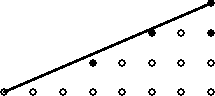
\includegraphics{pics/spin-377-pic-pics.pdf} \\
\caption{Generators in the $(\deg z, -ord_{P_i}(z))$ lattice}
\end{figure}

Also note that $e_j' + 2d = 7 + 2d \nmid 2 = e_i - e_j'$ for all
$i, j \in J = \{2, 3\}$ such that $j \neq i$ and for all $d \geq
0$. Thus, $s_{\sigma, J}(i, d) = \emptyset$ for each $i \in J$.
Furthermore, $\deg \lfloor e_i \halfcan \rfloor = \deg \lfloor 9
\halfcan \rfloor = 2 \lfloor \frac{4 * 9}{9} \rfloor + \lfloor
\frac{9}{3} \rfloor - 9 = 2$, so (Ad-iii) is satisfied and
$\sigma, J$ is admissible.

%Let $(-ord_{P_1}(x_j)$, $-ord_{P_2}(x_j)$, $-ord_{P_3}(x_j))$
%represent the pole orders of $x_i$ at each point. Then these generators
%must have pole orders $(1, 1, 1), (1, 2, 2), (2, 3, 2), (2, 2, 3)$
%respectively.

We can directly see that the relations are given in degrees $10$
and $14$. In particular, we have relations
\begin{align*}
	&a_1 x_{3, 1} x_{7, 2} + a_2 x_{3, 1} x_{7, 1} + a_3 x_{5, 1}^2 = 
	0 &\text{ in degree $10$} \\
	&b_1 x_{7, 2}^2 + b_2 x_{7, 1} x_{7, 2} + b_3 x_{7, 1}^2
	+ b_4 x_{3, 1}^3 x_{5, 1} = 0  &\text{ in degree $14$}
\end{align*}

\noindent
and note that $a_1$ and $b_1$ are both nonzero. If $a_1 = 0$, then we
have that
\[
	a_2 x_{3, 1} x_{7, 1} = -a_3 x_{5, 1}^2
\]

\noindent
However, $x_{3, 1} x_{7, 1}$ has pole orders $(3, 4, 3)$ and
$x_{5, 1}^2$ has pole orders $(2, 4, 4)$ so their
coefficients must be zero for this equality to hold. We have a
similar pole order consideration in forcing $b_1$ to be nonzero.

Let $I$ be the ideal generated by these relations in
$k[x_{7, 1}, x_{7, 2}, x_{5, 1}, x_{3, 1}]$. Under grlex with
$x_{3,1} \prec x_{5,1} \prec x_{7,1} \prec x_{7,2}$, the initial
ideal of $I$ is
\[
	in_\prec(I) = \langle x_{3, 1} x_{7, 2}, x_{7, 2}^2 \rangle
\]

\noindent
since $a_1$ and $b_1$ are nonzero.

To demonstrate that these two relations generate all 
relations, we show that $\dim_k (R')_d = \dim_k
(k[x_{3, 1}, x_{5, 1}, x_{7, 1}, x_{7, 2}] / in_\prec(I))_d$ for all degrees
$d \geq 0$. In particular, 

\begin{align*}
	\dim_k (k[x_{3, 1}, x_{5, 1}, x_{7, 1}, x_{7, 2}] / I)_d &=
	\dim_k (k[x_{3, 1}, x_{5, 1}, x_{7, 1}, x_{7, 2}]	/ in_\prec(I))_d \\
	&= \dim_k (k[x_{3, 1}, x_{5, 1}, x_{7, 1}, x_{7, 2}] / \langle x_{5, 1}^2,
	x_{7, 1}^2 \rangle
\end{align*}

\noindent
for all $d \geq 0$. But the fact $\dim_k (R')_d = \dim_k (k[x_{3, 1},
x_{5, 1}, x_{7, 1}, x_{7, 2}] / \langle x_{5, 1}^2,	x_{7, 1}^2 \rangle$ can
be checked by looking at the $k$-basis at each degree $d$.

Therefore, the canonical ring $R'$ has presentation $R' =
k[x_{7, 1}, x_{7, 2}, x_{5, 1}, x_{3, 1}] / I$ with
initial ideal $in_\prec(I)$ generated by quadratics under grlex
with $x_{7,1} \prec x_{7,2} \prec x_{5,1} \prec x_{3,1}$.
%These quadratics must also determine minimal generators for $I$ by
%Lemma ~\ref{lem:minimal_quadratic}.
Thus, $R'$ is generated up to degree $e = 7$ with relations up to
degree $2e = 14$, as desired.

%We can also see that $e_i > \deg z$ for any generator $z$ of $R'$
%since $e_i = 9 > e$ for all $i \in J$.
\end{example}

\begin{proof}[Proof of Lemma ~\ref{lem:g-0-admissible-cases}]
For the remaining cases, we can use a similar method to the one
used in Example ~\ref{ex:base-377} to find a presentation the
desired conditions.

The following table demonstrates that $R(\sx', 0, L')$ is
generated as a $k$-algebra by elements of degree at most $e$
with relations in degree at most $2e$ for each case. Also note
that in these cases, $e_i = e + 2 > \deg z$ for all $i \in J$
and any generator $z$ of $R'$.
\begin{longtable}
	{| c || c | c | c |}
	\caption{Genus 0 Non-effective Base Cases Generators/Relations}
	\label{table:g-0-base-cases-degrees}
	
	\tabularnewline
	
	\hline
	Case & Generator Degrees & Degrees of Relations & $e$\\
	\hline
	\hline

	(a) & \{3, 7, 9, 11\} & \{14, 18\} & 11\\	\hline

	(b) & \{3, 5, 7, 9\} & \{12, 14\}	& 9\\ \hline

	(c) & \{3, 5, 7, 7\} & \{10, 14\}	& 7\\ \hline
	
	(d) & \{3, 5, 5, 7\} & \{10, 12\}	& 7\\ \hline
	
	(e) & \{3, 5, 5, 7, 7\} & \{10, 10, 12, 12, 14\}	& 7\\ \hline
	
	(f) & \{3, 5, 5, 7, 7, 7\} & \{10, 10, 10, 12, 12, 12, 14, 14, 14\}	& 7\\ \hline

	(g) & \{3, 3, 4, 5\} & \{8, 9\} & 5\\ \hline
	
	(h) & \{3, 3, 4, 5, 5\} & \{8, 8, 9, 9, 10\} & 5\\ \hline
	
	(i) & \{3, 3, 4, 5, 5, 5\} &
	\{8, 8, 8, 9, 9, 9, 10, 10, 10\} & 5\\ \hline
	
	(j) & \{3, 3, 4, 5, 5, 5, 5\} &
	\{8, 8, 8, 8, 9, 9, 9, 9, 10, 10, 10, 10, 10, 10\} & 5\\ \hline

	(k) &	\{3, 3, 3, 4,	4, 5\} & \{6, 7, 7, 8, 8, 8, 9, 9, 10\} & 5\\ \hline
\end{longtable}

We can also always find a presentation for these cases such that
they satisfy (Ad-i) and (Ad-ii) and that $in_\prec(I')$ is
generated by products of two monomials. The procedure for
verifying these are similar to those for the given example.

Furthermore, each case always satisfies (Ad-iii) as demonstrated below.
Notice that the $e_i$ and $\{e_j' : j \neq i\}$ are equivalent
for any choice of $i \in J$ for these cases, so $\deg \lfloor e_i L
\rfloor$ and $\max_{d \geq 0} \#S_{(\sigma, J)}(i)$ are
independent of the choice of $i$.

\begin{longtable}
	{| c | c | c || c | c |}
	\caption{Genus 0 Non-Effective Base Cases (Ad-iii)}
	\label{table:g-0-base-cases-admissibility}
	
	\tabularnewline
	
	\hline
	Case & $\sigma$ & $J$ & $\deg \lfloor e_i L \rfloor$ &
	$\max_{d \geq 0} \#S_{(\sigma, J)}(i)$ \\
	\hline
	\hline

	(a) & $(0; 3, 3, 11; 0)$ & $\{3\}$ & 1 & 0 \\	\hline
	
	(b) & $(0; 3, 5, 9; 0)$ & $\{3\}$ & 1 & 0 \\ \hline
	
	(c) & $(0; 3, 7, 7; 0)$ & $\{3\}$ & 2 & 0 \\ \hline
	
	(d) & $(0; 5, 5, 7; 0)$ & $\{3\}$ & 1 & 0 \\ \hline
	
	(e) & $(0; 5, 7, 7; 0)$ & $\{2, 3\}$ & 2 & 0 \\ \hline

	(f) & $(0; 7, 7, 7; 0)$ & $\{1, 2, 3\}$ & 3 & 0 \\ \hline

	(g) & $(0; 3, 3, 3, 5; 0)$ & $\{4\}$ & 2 & 0 \\ \hline
	
	(h) & $(0; 3, 3, 5, 5; 0)$ & $\{3, 4\}$ & 3 & 0 \\ \hline
	
	(i) & $(0; 3, 5, 5, 5; 0)$ & $\{2, 3, 4\}$ & 4 & 0 \\ \hline
	
	(j) & $(0; 5, 5, 5, 5; 0)$ & $\{1, 2, 3, 4\}$ & 5 & 0 \\ \hline

	(k) & $(0; 3, 3, 3, 3, 3; 0)$ & $\{1, 2, 3, 4, 5\}$ & 5 & 0 \\ \hline
\end{longtable}

Thus, all of the cases are admissible and satisfy the additional
desired conditions.
\end{proof}

Now we can use Lemma ~\ref{lem:sat-3}, Lemma
~\ref{lem:raise-stacky-order}, and Corollary
~\ref{cor:raise-stacky-order} inductively on the cases of Table
~\ref{table:g-0-base-cases} to obtain the desired bounds on the
generator and relation degrees for log spin canonical rings of
genus 0 curves. This process will be carried out in Subsection
~\ref{ssec:g-0-main}.


%Through the application of two inductively adding 
%points via Lemma ~\ref{lem:sat-3} and inductively raising
%stabilizer orders via Lemma ~\ref{lem:raise-stacky-order},
%we obtain Theorem ~\ref{thm:g-0-main} for any
%log spin curve $(\sx, \Delta, L)$ with
%signature $\sigma$ covered by this induction process.
%In particular, this induction process covers all signatures $\sigma
%= (0; e_1, \ldots, e_r; 0)$ such that either $r \geq 5$ or
%for some listed base case $(\sigma', J)$ with $\sigma' = (0; e_1',
%\ldots, e_r'; 0)$, $e_i \geq e_i'$ for all $i$.
%Before we prove the main theorem, we describe the cases not be
%covered by induction.


\ssec{Exceptional Cases}
\label{ssec:g-0-exceptional}
In this subsection, we describe the cases that would not be covered by induction.
We present the explicit generators and relations for the remaining
cases given by signatures in the finite set

\begin{align*}
	S &:= \{(0; 3, 3, k; 0) : 3 \leq k \leq 9 \text{ odd}\} \\
		&\cup \{(0; 3, 5, 5; 0) ,(0; 3, 5, 7; 0), (0; 5, 5, 5; 0), (0; 3, 3, 3, 3; 0)\}
\end{align*}

\noindent
and in particular describe the only exceptions to Theorem ~\ref{thm:main}
in the case $g = 0$.

\begin{longtable}
	{| c || c | c | c |}
	\caption{Genus 0 Exceptional Cases}
	\label{table:g-0-exceptional}
	
	\tabularnewline
	
	\hline
	Signature & Generator Degrees & Degrees of Relations & $e$ \\
	\hline
	\hline

	$(0; 3, 3, 3; 0)$ & $\{3\}$ & $\emptyset$ & $3$ \\	\hline

	$(0; 3, 3, 5; 0)$ & $\{3, 10, 15\}$ & $\{30\}$ & $5$ \\	\hline
	
	$(0; 3, 3, 7; 0)$ & $\{3, 7, 12\}$ & $\{24\}$ & $7$ \\	\hline
	
	$(0; 3, 3, 9; 0)$ & $\{3, 7, 9\}$ & $\{21\}$ & $9$ \\	\hline
	
	$(0; 3, 5, 5; 0)$ & $\{3, 5, 10\}$ & $\{20\}$ & $5$ \\	\hline
	
	$(0; 3, 5, 7; 0)$ & $\{3, 5, 7\}$ & $\{17\}$ & $7$ \\	\hline
	
	$(0; 5, 5, 5; 0)$ & $\{3, 5, 5\}$ & $\{15\}$ & $5$ \\	\hline
	
	$(0; 3, 3, 3, 3; 0)$ & $\{3, 3, 4\}$ & $\{12\}$ & $3$ \\	\hline
\end{longtable}

\begin{rem}
These cases give all of the exceptions to the $e$ and $2e$ bounds on
the generator and relation degree. Notice that each of these
exceptional cases, apart from $(0; 3, 5, 7; 0)$, corresponds to a
signature with saturation not equal to
3, 5, or 9. as seen in Table ~\ref{table:g-0-sat}. Heuristically,
these exceptional saturations can be viewed as ``forcing'' generators
(and thus relations) to lie in higher degrees than expected.
\end{rem}

\ssec{Main Theorem for Genus Zero}
\label{ssec:g-0-main}
Now we can combine this.

\begin{thm}
\label{thm:g-0-main}
Let $(\sx, \Delta, \halfcan)$ log spin curve,
so that $\sx$ has signature $\sigma = (0; e_1, \ldots, e_r; \delta)$.
Then, the canonical ring

\begin{align*}
	R(\sx, \Delta, \halfcan) = \bigoplus_{d = 0}^\infty H^0(\sx, \lfloor d L \rfloor)
\end{align*}

\noindent
is generated as a $k$-algebra by elements of degree at most $e =
\max(5, e_1, \ldots, e_r)$ and has relations in degree at most $2e$,
so long as $\sigma$ does not lie in the finite list of exceptional
cases listed in Table ~\ref{table:g-0-exceptional}.
\end{thm}

\begin{proof}
If $\sx$ has no stacky points, then we can assume that $L \sim
n \cdot \infty$ with $n \in \BZ$. This is the classical
case which is done, with $L$ replaced by $K$, by Voight and
Zureick-Brown ~\cite[Section 4.2]{vzb:stacky}.

First, let us consider the case when $\delta \geq 2$. In any such case,
$\lfloor \halfcan \rfloor$ is an effective divisor and the conditions
of Lemma ~\ref{lem:sat-1} are satisfied. Thus, we can apply
the Lemma ~\ref{lem:sat-1} inductively on the classical case with no stacky points
to get that $R(\sx, \Delta, \halfcan)$ is generated up to degree $e$
with relations generated up to degree $2e$.

It only remains to deal with the case $\delta = 0$, so $\halfcan$ is not effective.
Let $\sigma = (0; e_1, \ldots, e_r; 0)$ be a signature with $r > 0$
so that $\sigma$ is not one of the exceptional cases in Table
~\ref{table:g-0-exceptional}. Note that if $r < 3$, then $\deg 
\lfloor d \halfcan \rfloor < 0$ for all $d \geq 0$ so we have the
trivial case where $R(\sx, \Delta, \halfcan) = k$. Thus, we now
only consider the cases with $r \geq 3$.

If $r > 5$, then we can use Lemma
~\ref{lem:sat-3} to add stacky points with
stabilizer order $3$ to case (k) of Table
~\ref{table:g-0-base-cases}, which corresponds to $\sigma
= (0; 3, 3, 3, 3, 3; 0), J = \{1, 2, 3, 4, 5\}$. This case
satisfies the conditions of Lemma
~\ref{lem:sat-3} (recall from Table ~\ref
{table:g-0-sat} that $\sat(\Eff(\sigma)) = 3$), and the
immediate consequence of parts (a) and (c) of Lemma
~\ref{lem:sat-3} is that any $R(\sx', \Delta,
\halfcan')$ corresponding to signatures $\sigma'$ with ramification
orders all equal to $3$ for any $r > 5$ is generated up to
degree $e' := \max(5, e_1', \ldots, e_r')$ with relations generated
up to degree $2e'$. Furthermore, these cases satisfy all of the
conditions of Lemma ~\ref{lem:raise-stacky-order}. Now we can
apply Corollary ~\ref{cor:raise-stacky-order} to deduce that
$R(\sx, \delta, \halfcan)$ is generated up to degree $e :=
\max(5, e_1, \ldots, e_r)$ with relations generated up to degree
$2e$.

If $r \leq 5$ and $\sigma$ is not one of the exceptional cases,
then we may similarly apply Lemma ~\ref{lem:g-0-admissible-cases} and
Corollary ~\ref{cor:raise-stacky-order} to an appropriate base case
from Table ~\ref{table:g-0-base-cases} and deduce that $R(\sx,
\delta, \halfcan)$ is generated up  to degree $e := \max(5, e_1,
\ldots, e_r)$ with relations generated up to degree $2e$.
 \end{proof}

\section{Further Research}
\label{sec:further-questions}

This paper leaves open many directions for further research.

\begin{enumerate}
	\item In the case $g \geq 2$, Proposition ~\ref{prop:relation_11} gives a bound on the degree of generators of the relations of a log spin canonical ring $R_L$. Additionally, by Remark ~\ref{rem:relations_generation_ten}, any curve of genus 2 with half canonical divisor $L = P$ has spin canonical ring $R_L$ with relations in degree 10. This raises the question of whether the bound of 11 on the degree of the relations in $R_L$ can be reduced to $10$. In particlar, we make the following conjecture.
\begin{conjecture}
\label{conj:relations-10}
If $X$ is a curve of genus $g \geq 2$ and $L \in \di X$ with $2L \sim K,$ the ideal of relations in $R_L$ is generated in degree at most $10$. More precisely, if $x_1,\ldots, x_n$ is a minimal set of generators for $R_L$ and $\phi:k[y_1,\ldots, y_n] \rightarrow R_L, y_i \mapsto x_i,$ then $I_L := \ker \phi$, is generated in degree at most 10. 
\end{conjecture}
Note that in the case $\dim L \geq 2$ and $L$ is basepoint-free, by Neves ~\cite[Proposition III.12]{neves:halfcan}, $I_L$ is generated in degree at most 8. Additionally, if Conjecture ~\ref{conj:relations-10} were true, by Theorem ~\ref{thm:main} we would immediately obtain the following corollary, providing a more concise statement than that of Theorem ~\ref{thm:main}.
\begin{cor}
\label{cor:main-refined}
Let $(\sx,\Delta,L)$ be a log spin curve over a perfect field $k$ with signature $(g;e_1,\ldots, e_r;\delta)$ and let $R_L$ be the log canonical ring. Suppose Conjecture ~\ref{conj:relations-10}. Then, $R_L$ is generated in degree at most $e = \max(5,e_1,\ldots, e_r)$ with relations in degree at most $2e,$ apart from a finite list of exceptions.
\end{cor}
	\item Another direction for further research is to extend the results of this paper to divisors $D \in \di \sx$ on a stacky curve $\sx,$ where $nD \sim K.$ The canonical rings of such divisors would translate to rings of fractional weight modular forms. As defined in Adler and Ramanan, immediately following \cite[Corollary 24.5]{adler:moduli}, a {\bf modular form of fractional weight} $\frac{2a}{n}$ on $X(p)$ is a section of a line bundle $\eta$ so that there exists a line bundle $\gamma$ with $\gamma^{\otimes a} \cong \eta$ and $\gamma^{n} \cong \Omega_{X(p)}^1$. Adler and Ramanan \cite[Appendix 2]{adler:moduli} construct an explicit basis of weight $\frac{4}{5}$ modular forms for $X(11)$. Fractional modular forms also make an apperance in Milnor \cite[$\mathsection$ 6]{milnor:fractional-weight}. In this work, Milnor shows that for a triangle group $\Gamma$ of signature $(0; e_1,e_2,e_3; 0)$ there exist generators $f_1,f_2,f_3$ of a certain ring of fractional weight modular forms, satisfying $f_1^{e_1}+f_2^{e_2}+f_3^{e_3} = 0$. 

Having motivated the importance of fractional weight modular forms, we pose the following question:

\begin{question}
\label{ques:fractional-weight}
If $\sx$ is a stacky curve and $D \in \di \sx$ with $nD \sim K,$ where $K$ is the canonical divisor of $\sx$, can one bound the degrees of generators and relations of $R_D$?
\end{question}
Note that that the above question is answered affirmatively in the case that $\sx$ has genus $0$ and $D$ is effective, as follows by inductively applying Lemma ~\ref{lem:sat-1}: If $\sx$ has signature $(g;e_1, \ldots, e_r; \delta)$ then $D$ is generated in degree at most $e = \max(e_1, \ldots, e_r)$ with relations in degree at most $2e$. Additionally, it may be possible to modify the proof of Lemma ~\ref{lem:raise-stacky-order} to extend to the setting of fractional weight modular forms. Given suitable generalizations of these lemmas, one may be able to approach the problem of finding generators and relations for fractional weight modular forms using techniques similar to those in this paper.
	\item In Voight and Zureick Brown \cite[Definition 2.2.7]{vzb:stacky}, the notion of a generic initial ideal is defined, which encapsulates the idea of whether the relations for $R_L$ are generically chosen, in a precise sense. The proof of Theorem ~\ref{thm:main} decidedly does not yield a generic initial ideal, as generators and relations are constructed in a highly nongeneric manner. In particular, Lemma ~\ref{lem:raise-stacky-order} constructs generators with non-maximal pole orders at certain points, making the relations non-generic. 
\begin{question}
\label{ques:generic-initial}
If $(\sx,\Delta,L)$ is a log spin curve with signature $\sigma$, does there exist a function $\sigma \mapsto d(\sigma)$ so that the generic initial ideal {\rm(} with some specified ordering{\rm)} is generated in degree at most $d(\sigma)$? Can one write down the generic initial ideal explicitly?
\end{question}
	\item As noted in Remark ~\ref{rem:explicit-generators}, the proof of Theorem ~\ref{thm:main} given in this paper gives an explicit procedure for computing the generators and relations of $R_L$ when the genus of $\sx$ is $0$ or $1$.
\begin{question}
\label{ques:algorithm}
Can one give an algorithm for explicitly computing the generators and relations for an arbitrary genus $g \geq 2$ curve?
\end{question}
Suppose the generators and relations of $R_{L_X}$ are known, where $(\sx, \Delta, L)$ is a spin canonical ring, $X$ is the coarse space of $\sx$, and $L_X \leq L$ is a half canonical divisor of $X$. In this case our proof of Theorem ~\ref{thm:main} yields an algorithm for determining the generators of $L$. This raises the following Petri-like question:
\begin{question}
\label{ques:half-canonical-petri}
Given a {\rm(}non-stacky {\rm)} curve $X$ and a half canonical divisor $L \in \di X$, can one write down a set of minimal generators and minimal relations for $R_L$? If so, can one give the generic ideal of $R_L$ or the generic initial ideal of $R_L$, as defined in Voight and Zureick Brown \cite[Definition 2.2.7]{vzb:stacky}?
\end{question}
In particular, if Question ~\ref{ques:half-canonical-petri} were answered affirmatively one would be able to write down explicit generators and relations for $R_L$ on a stacky curve, essentially by inductively applying Lemma ~\ref{lem:raise-stacky-order}.
	\todo{This last one doesn't seem particularly interesting. Should we remove it?}
	\item While Theorem ~\ref{thm:main} gives a minimal set of generators for the log spin canonical ring $R_L,$ the set of relations is not minimal. In many of the $g = 0$ and $g=1$ cases, it is not too difficult to see that our inductive procedure also yields a minimal set of relations for $R_L$. One might investigate whether the generators and relations given by the inductive proof of Theorem ~\ref{thm:main} are always minimal.
	\end{enumerate}

%%%%%%%%%%%%%%%%%%%%%%%%% Acknowledgements %%%%%%%%%%%%%%%%%%%%%%%%%%%%

\section{Acknowledgments}
We are grateful to David Zureick-Brown for introducing us to this
field of study, providing incredibly helpful guidance, and being an
excellent project mentor. We also thank Ken Ono and the Emory University
Number Theory REU for arranging our project and providing a great
environment for mathematical learning and collaboration. Finally, we
gratefully acknowledge that our research was financially supported by
NSF Grant Award Number 1250467 via the Emory University Number Theory REU.
We deeply appreciate all of the support that has made our work possible.

%%%%%%%%%%%%%%%%%%%%%%%%%%%% References %%%%%%%%%%%%%%%%%%%%%%%%%%%%%%%

\nocite{*}
\bibliography{bibliography}{}
\bibliographystyle{plain}

\end{document}